%%%%%%%%%%%%%%%%%%%%%%%%%%%%%%%%%%%%%%%%%%%%%%%%%%%%%%%%%%%%%%%%%%%%%%%%%%%%%%%
% Uni Duesseldorf
% Lehrstuhl fuer Datenbanken and Informationssysteme
% Vorlage fuer Bachelor-/Masterarbeiten
% Optimiert fuer den Original-Latex-Kompiler LATEX.EXE (LaTeX=>PS=>PDF)
% Version 1.4 - 2.3.2010
%%%%%%%%%%%%%%%%%%%%%%%%%%%%%%%%%%%%%%%%%%%%%%%%%%%%%%%%%%%%%%%%%%%%%%%%%%%%%%%

%%%%%%%%%%%%%%%%%%%%%%%%%%%%%%%%%%%%%%%%%%%%%%%%%%%%%%%%%%%%%%%%%%%%%%%%%%%%%%%
%%%%%%%%%%% BEGINN EINSTELLUNG FUER DIE ARBEIT. UNBEDINGT ERFORDERLICH! %%%%%%%
%%%%%%%%%%%%%%%%%%%%%%%%%%%%%%%%%%%%%%%%%%%%%%%%%%%%%%%%%%%%%%%%%%%%%%%%%%%%%%%
% Geben Sie Ihren Namen hier an
\newcommand{\bearbeiter}{Alina Elterman}

% Geben Sie hier den Titel Ihrer Arbeit an
\newcommand{\titel}{Game-theoretic Analysis of the Strategyproofness of Cake-cutting Protocols}

% Geben Sie das Datum des Beginns and Ende der Bachelorarbeit ein
\newcommand{\beginndatum}{05. September 2011}
\newcommand{\abgabedatum}{05.~Dezember~2011}

% Geben Sie die Namen des Erst- and Zweitgutachters an
\newcommand{\erstgutachter}{Prof. Dr.~J\"org Rothe}
\newcommand{\zweitgutachter}{Prof. Dr.~Peter Kern}

% Falls Sie die Arbeit zweiseitig ausdrucken wollen,
% benutzen Sie die folgende Zeile mit
% \AN fuer zweiseitigen Druck
% \AUS fuer einseitigen Druck
\newcommand{\zweiseitig}{\AUS}

% Falls die Arbeit in englischer Sprache verfasst 
% werden soll, dann benutzen Sie die folgende Zeile mit
% englisch fuer englische Sprache
% deutsch fuer deutsche Sprache
\newcommand{\sprache}{englisch}
%%%%%%%%%%%%%%%%%%%%%%%%%%%%%%%%%%%%%%%%%%%%%%%%%%%%%%%%%%%%%%%%%%%%%%%%%%%%%%%%%
%%%%%%%%%%%%%%%%%%%%%%%%%%%%%%% ENDE EINSTELLUNGEN %%%%%%%%%%%%%%%%%%%%%%%%%%%%%%
%%%%%%%%%%%%%%%%%%%%%%%%%%%%%%%%%%%%%%%%%%%%%%%%%%%%%%%%%%%%%%%%%%%%%%%%%%%%%%%%%

% Die folgende Zeile NICHT EDITIEREN oder loeschen
% (Zum Ab�ndern der BA-Vorlage in eine MA-Vorlage muessen sie
% jedoch die Datei titelmakros1.tex selbst editieren.)
%%%%%%%%%%%%%%%%%%%%%%%%%%%%%%%%%%%%%%%%%%%%%%%%%%%%%%%%%%%
% Obere Titelmakros. Editieren Sie diese Datei nur, wenn
% Sie sich ABSOLUT sicher sind, was Sie da tun!!!
% (Z.B. zum Abaendern der BA-Vorlage in eine MA-Vorlage)
% Uni Duesseldorf
% Lehrstuhl fuer Datenbanken und Informationssysteme
% Version 2.2 - 2.3.2010
%%%%%%%%%%%%%%%%%%%%%%%%%%%%%%%%%%%%%%%%%%%%%%%%%%%%%%%%%%%
\newcommand{\AN}{twoside}
\newcommand{\AUS}{}
%\newcommand{\englisch}{}
%\newcommand{\deutsch}{\usepackage[german]{babel}}

%% Die folgenden auskommentierten Optionen dienen der automatischen
%% Erkennung des Latex-Kompilers und dem Setzen der davon abh�ngigen
%% Einstellungen. Bei Problem z.B. mit dem Einbinden von verschiedenen
%% Grafiktypen bei Verwendung von PdfLatex oder Latex, einfach die
%% verschiedenen \usepackage(s) ausprobieren. (Mit diesen Einstellungen
%% funktionierte diese Vorlage bei der Verwenundg von latex.exe als
%% Kompiler bei den meisten Studierenden.)

%\newif\ifpdf \ifx\pdfoutput\undefined
%\pdffalse % we are not running pdflatex
%\else
%\pdfoutput=1 % we are running pdflatex
%\pdfcompresslevel=9 % compression level for text and image;
%\pdftrue \fi

\documentclass[11pt,a4paper, \zweiseitig]{article}



%\usepackage[iso]{umlaute}
\usepackage[latin1]{inputenc}
\usepackage{palatino} % palatino Schriftart
%\usepackage{makeidx} % um ein Index zu erstellen
\usepackage{tocbibind}
\usepackage[T1]{fontenc} %fuer richtige Trennung bei Umlauten
\usepackage{fancybox} % fuer die Rahmen
\usepackage{shortvrb}
\usepackage{ifthen}
\ifthenelse{\equal{\sprache}{deutsch}}{\usepackage[ngerman]{babel}}{}

\usepackage{lmodern} 
\usepackage{amsmath}
\usepackage{amssymb}
\usepackage{pdfpages}
\usepackage{hyperref}
%\usepackage{fancyheadings}
\usepackage{fancyhdr}
\usepackage{amsfonts}
\usepackage{amsthm}
\usepackage{color}
\usepackage{stmaryrd}
\usepackage{nomencl}
\usepackage[normalem]{ulem} 
\newcommand{\markup}[1]{\uline{#1}}
% Befehl umbenennen in abk
\let\abk\nomenclature

\usepackage{a4wide} % ganze A4 Weite verwenden

%\ifpdf
%\usepackage[pdftex,xdvi]{graphicx}
%\usepackage{thumbpdf} %thumbs fuer Pdf
%\usepackage[pdfstartview=FitV]{hyperref} %anklickbares Inhaltsverzeichnis
%\else
\usepackage[dvips,xdvi]{graphicx}
\usepackage{hyperref} %anklickbares Inhaltsverzeichnis
%\fi

%%%%%%%%%%%%%%%%%%%%%%% Massangaben fuer die Arbeit %%%%%%%%%%%%%%%
\setlength{\textwidth}{15cm}

\setlength{\oddsidemargin}{35mm}
\setlength{\evensidemargin}{25mm}

\addtolength{\oddsidemargin}{-1in}
\addtolength{\evensidemargin}{-1in}

%\makeindex
% Umgebungen f"ur S�tze usw.
\newtheorem*{bemerkung*}{Bemerkung}
\newtheorem*{defi}{Definition}
\newtheorem*{defi*}{Definition}
\newtheorem*{bezeichnungen}{Bezeichnungen}
\newtheorem*{fakt}{Fakt}
\newtheorem*{beispiel}{Beispiel}
\newtheorem*{bsp}{Beispiel}
\newtheorem*{beispiel*}{Beispiel}
\newtheorem*{satz}{Satz}
\newtheorem*{satz*}{Satz}
\newtheorem*{lem}{Lemma}
\newtheorem*{protokoll*}{Protokoll}
\newtheorem*{idee}{Idee}

%definition of new commands
\newcommand{\DGEF}{\text{\textbf{DGEF}}}

\begin{document}

%\setcounter{secnumdepth}{4} %Nummerieren bis in die 4. Ebene
%\setcounter{tocdepth}{4} %Inhaltsverzeichnis bis zur 4. Ebene

\pagestyle{headings}

\sloppy % LaTeX ist dann nicht so streng mit der Silbentrennung
\MakeShortVerb{\�}

\parindent0mm
\parskip0.5em


{
\textwidth170mm 
\oddsidemargin30mm 
\evensidemargin30mm 
\addtolength{\oddsidemargin}{-1in}
\addtolength{\evensidemargin}{-1in}

\parskip0pt plus2pt

% Die Raender muessen eventuell fuer jeden Drucker individuell eingestellt
% werden. Dazu sind die Werte fuer die Abstaende `\oben' und `\links' zu
% aendern, die von mir auf jeweils 0mm eingestellt wurden.

%\newlength{\links} \setlength{\links}{10mm}  % hier abzuaendern
%\addtolength{\oddsidemargin}{\links}
%\addtolength{\evensidemargin}{\links}

\begin{titlepage}
\vspace*{-1.5cm}
  \raisebox{17mm}{
    \begin{minipage}[t]{70mm}
      \begin{center}
        %\selectlanguage{german}
        {\Large INSTITUT F�R INFORMATIK\\}
        {\normalsize
          Lehrstuhl f�r Komplexit\"atstheorie und Kryptologie
\\
        }
        \vspace{3mm}
        {\small Universit�tsstr. 1 \hspace{5ex} D--40225 D�sseldorf\\}
     \end{center}
    \end{minipage}
  }
  \hfill
  
\includegraphics[width=130pt]{bilder/HHU_Logo}
  \vspace{14em}

% Titel
  \begin{center}
      	\baselineskip=55pt
    	\textbf{\huge \titel}
  	 	\baselineskip=0 pt
   \end{center}

  %\vspace{7em}

\vfill

% Autor
  \begin{center}
    \textbf{\Large
      \bearbeiter
    }
  \end{center}

  \vspace{35mm}
 
% Pr�fungsordnungs-Angaben
  \begin{center}
    %\selectlanguage{german}
    
%%%%%%%%%%%%%%%%%%%%%%%%%%%%%%%%%%%%%%%%%%%%%%%%%%%%%%%%%%%%%%%%%%%%%%%%%
% Ja, richtig, hier kann die BA-Vorlage zur MA-Vorlage gemacht werden...
%%%%%%%%%%%%%%%%%%%%%%%%%%%%%%%%%%%%%%%%%%%%%%%%%%%%%%%%%%%%%%%%%%%%%%%%%
    {\Large Bachelorarbeit}

    \vspace{2em}

    \begin{tabular}[t]{ll}
      Beginn der Arbeit:& \beginndatum \\
      Abgabe der Arbeit:& \abgabedatum \\
      Gutachter:         & \erstgutachter \\
                         & \zweitgutachter \\
    \end{tabular}
  \end{center}

\end{titlepage}

}

%%%%%%%%%%%%%%%%%%%%%%%%%%%%%%%%%%%%%%%%%%%%%%%%%%%%%%%%%%%%%%%%%%%%%
\clearpage
\begin{titlepage}
  ~                % eine leere Seite hinter dem Deckblatt
\end{titlepage}
%%%%%%%%%%%%%%%%%%%%%%%%%%%%%%%%%%%%%%%%%%%%%%%%%%%%%%%%%%%%%%%%%%%%%
\clearpage
\begin{titlepage}
\vspace*{\fill}

\section*{Erkl�rung}

%%%%%%%%%%%%%%%%%%%%%%%%%%%%%%%%%%%%%%%%%%%%%%%%%%%%%%%%%%%
% Und hier ebenfalls ggf. BA durch MA ersetzen...
%%%%%%%%%%%%%%%%%%%%%%%%%%%%%%%%%%%%%%%%%%%%%%%%%%%%%%%%%%%

Hiermit versichere ich, dass ich diese Bachelorarbeit
selbstst�ndig verfasst habe. Ich habe dazu keine anderen als die
angegebenen Quellen und Hilfsmittel verwendet.

\vspace{25 mm}

\begin{tabular}{lc}
D�sseldorf, den \abgabedatum \hspace*{2cm} & \underline{\hspace{6cm}}\\
& \bearbeiter
\end{tabular}

\vspace*{\fill}
\end{titlepage}

%%%%%%%%%%%%%%%%%%%%%%%%%%%%%%%%%%%%%%%%%%%%%%%%%%%%%%%%%%%%%%%%%%%%%
% Leerseite bei zweiseitigem Druck
%%%%%%%%%%%%%%%%%%%%%%%%%%%%%%%%%%%%%%%%%%%%%%%%%%%%%%%%%%%%%%%%%%%%%

\ifthenelse{\equal{\zweiseitig}{twoside}}{\clearpage\begin{titlepage}
~\end{titlepage}}{}

%%%%%%%%%%%%%%%%%%%%%%%%%%%%%%%%%%%%%%%%%%%%%%%%%%%%%%%%%%%%%%%%%%%%%
\clearpage
\begin{titlepage}

\section*{\ifthenelse{\equal{\sprache}{deutsch}}{Zusammenfassung}{Abstract}}


%%%%%%%%%%%%%%%%%%%%%%%%%%%%%%%%%%%%%%%%%%%%%%%%%%%%%%%%%%%%%%%%%%%%%%%%%%%%%%%%%
%%%%%%%%%%%%%%%%%%%%%%%%%%%% BEGINN ZUSAMMENFASSUNG %%%%%%%%%%%%%%%%%%%%%%%%%%%%%
%%%%%%%%%%%%%%%%%%%%%%%%%%%%%%%%%%%%%%%%%%%%%%%%%%%%%%%%%%%%%%%%%%%%%%%%%%%%%%%%%
In cake-cutting a protocol instructs the participants how to divide a resource between\\them in a satisfactory manner. A part of those instructions, namely the strategies,\\are optional and their advantage can be examined. If this is not the case, the players have no intention to use that protocol, which can be overruled in this case. Otherwise the protocol is strategyproof.\\Game Theory is designed to determine better strategies. By using a game-theoretic illustration of the cake-cutting problem it is possible to compare all strategies.\\The strategy recommended by the protocol appears to be the best one in the well-known protocols with one exception.  
%%%%%%%%%%%%%%%%%%%%%%%%%%%%%%%%%%%%%%%%%%%%%%%%%%%%%%%%%%%%%%%%%%%%%%%%%%%%%%%%%
%%%%%%%%%%%%%%%%%%%%%%%%%%%%% ENDE ZUSAMMENFASSUNG %%%%%%%%%%%%%%%%%%%%%%%%%%%%%%
%%%%%%%%%%%%%%%%%%%%%%%%%%%%%%%%%%%%%%%%%%%%%%%%%%%%%%%%%%%%%%%%%%%%%%%%%%%%%%%%%

% Die folgende Zeile NICHT EDITIEREN oder loeschen
%%%%%%%%%%%%%%%%%%%%%%%%%%%%%%%%%%%%%%%%%%%%%%%%
% Untere Titelmakros. Editieren Sie diese Datei nur, wenn Sie sich
% ABSOLUT sicher sind, was Sie da tun!!!
%%%%%%%%%%%%%%%%%%%%%%%%%%%%%%%%%%%%%%%%%%%%%%%
\vspace*{\fill}
\end{titlepage}

%%%%%%%%%%%%%%%%%%%%%%%%%%%%%%%%%%%%%%%%%%%%%%%%%%%%%%%%%%%%%%%%%%%%%
% Leerseite bei zweiseitigem Druck
%%%%%%%%%%%%%%%%%%%%%%%%%%%%%%%%%%%%%%%%%%%%%%%%%%%%%%%%%%%%%%%%%%%%%
\ifthenelse{\equal{\zweiseitig}{twoside}}
  {\clearpage\begin{titlepage}~\end{titlepage}}{}
%%%%%%%%%%%%%%%%%%%%%%%%%%%%%%%%%%%%%%%%%%%%%%%%%%%%%%%%%%%%%%%%%%%%%
\clearpage 
\tableofcontents
\thispagestyle{empty}
%\enlargethispage{\baselineskip}
\clearpage \setcounter{page}{1}
%%%%%%%%%%%%%%%%%%%%%%%%%%%%%%%%%%%%%%%%%%%%%%%%%%%%%%%%%%%%%%%%%%%%%
% Leere Seite, falls Inhaltsverzeichnis mit ungerader Seitenzahl und 
% doppelseitiger Druck
%%%%%%%%%%%%%%%%%%%%%%%%%%%%%%%%%%%%%%%%%%%%%%%%%%%%%%%%%%%%%%%%%%%%%
\ifthenelse{ \( \equal{\zweiseitig}{twoside} \and \not \isodd{\value{page}} \)}
	{\pagebreak \thispagestyle{empty} \cleardoublepage}{\clearpage}



%%%%%%%%%%%%%%%%%%%%%%%%%%%%%%%%%%%%%%%%%%%%%%%%%%%%%%%%%%%%%%%%%%%%%
%%%%%%%%%%%%%%%%%%%%%%%%% BEGINN TEXTTEIL %%%%%%%%%%%%%%%%%%%%%%%%%%%
%%%%%%%%%%%%%%%%%%%%%%%%%%%%%%%%%%%%%%%%%%%%%%%%%%%%%%%%%%%%%%%%%%%%%
\section{Introduction}
It is Christmas party in the cakes4people agency. Everybody is waiting expectantly on the big promised cake at the end of the party. In the past years those cakes have been spectacular. A lot of different cake layers, different fruits on top and even chocolate sprinkles over parts of the cake have been so delicious. So it's no wonder that everyone wants to get as much as possible of this culinary treat, and especially of their individual favourite part. Nevertheless, the people do not want to penalise their colleagues.\\A new employee is also celebrating with the group. Rumors have been told a lot about him, but no one has managed to assess him or his preferences properly. Nevertheless, he also takes part in the big cake division. He even wants to change the allocation procedure. He promises that everyone can keep their wishes private, each of them just needs to make a couple of simple decisions and will get their best possible share.\\But the people become suspicious. Different questions occur in their minds: ''What if he has a strategy he is not telling us about, which promises him a better piece? What if he is lying about his preferences? Why should we trust him?''
The chief sees the mistrust and knows how to reassure the people. He is a game theory enthusiast and promises to show them that the proposed procedure is strategyproof. Hereby, only by taking actions truthful a participant can always get his best possible piece.\\
Strategyproofness of an allocation procedure ...
\begin{comment}
%Erklären was ist FAIR DIVISION\\ Kuchen geschnitten, nicht geteilt Krimi
%%A desirable property for cake-cutting protocols is strategy-proofness [6]. A protocol is strategy-proof if there is no incentive for any player to lie about his utility function. A protocol defines what to do for each player pi according to its utility function i. Since i is unknown to any other player, pi can execute some action that differs from the protocol’s definition (by pretending that pi ’s utility function is  ′i(≠ i)). If pi obtains more utility by lying about his utility function, the protocol is not strategy-proof. If a protocol is not strategy-proof,each player has to consider what to do and the result might differ from the intended result. If a protocol is strategy-proof, the best policy for each player is simply observing the rule of the protocol.%%
%(kein sehr guter anfang gez. herr rothe)Strategic play, cheating, incentive compatible, risk aversion, truthfulness, strategyproof and a lot more. All of them are keywords of whether an algorithm can resist the actions of selfish players and their greediness.
%Cake-cutting is part of interdisciplinary fields like economics, mathematics, operations research, political and computer science. Game theory is fulfilling the same property. Except for this fact, they have hardly something in common. While cake cutting is about fair division of a heterogeneous divisible good, where the studies are especially concentrated on types of fairness, game theory studies the strategies people use when making decisions.\\
%The role of strategies has not been widely researched yet in the context of cake cutting. But their importance is indisputable, with respect to fairness. Imagine the following situation:
%Example Cost Sharing from Algorithmic GT Noam Nissan chap. 15
%\begin{itemize}
%\item{division of sports tickets, health resources, computer networking resources, voting power, intellectual property licenses, costs for environmental improvements, etc}
%\item{formalize fairness, including max-min fairness, proportional fairness, envy-free fairness, etc. which may or may not lead to stable allocations in the sense of say Nash Equilibrium, or strong Nash Equilibrium}
%\end{itemize}
%Es werden Auswirkungen von nicht ehrlichen Strategien auf die Gerechtigkeit von Protokollen betrachtet. Der approach der Neidfreiheit ist zu stark, da kein finite bounded Protokoll f"ur n >3 (>4 f"ur allgemein) bekannt ist. Dagegen w"are der approach der Proportionaltit"at zu schwach, $\dots$. Das notwendige Mittelmaß liefert der DGEF und so fällt der Focus dieser Arbeit auf die Möglichkeit den DGEF eines Protokolles durch unehrliche Strategien zu erhöhen. Die Analyse erfolgt mittels Spieltheorie.\\
%\newline
%$\cdot$ Able to show that the only strategy promising a fair share is the recommended one.
\end{comment}
\pagebreak
%%%%%%%%%%%%%%%%%%%%%%%%%%%%%%%%%%%%%%%%%%%%%%%%%%%%%%%%%%%%%%%%%%%%%%%%%%%%%%%%%%%%%%%%%%%%%%%%%%%%%%%%%%%%%%%%
%%%%%%%%%%%%%%%%%%%%%%%%%%%%%%%%%%%%%%%%%%%%%%%%%%%%%%%%%%%%%%%%%%%%%%%%%%%%%%%%%%%%%%%%%%%%%%%%%%%%%%%%%%%%%%%%
%%%%%%%%%%%%%%%%%%%%%%%%%%%%%%%%%%%%%%%%%%%%%%%%%%%%%%%%%%%%%%%%%%%%%%%%%%%%%%%%%%%%%%%%%%%%%%%%%%%%%%%%%%%%%%%%
\section{Preliminaries}
\subsection{Basics of Cake-cutting}
It is necessary to define the components and challenges of cake-cutting. But first, what exactly is cake-cutting about? It involves a set of $n \in \mathbb{N}$ players $P_n=\{p_1,\ldots,p_n\}$. It is assumed that each of them wants to get as much as possible of the divided resource. The goal is to find an allocation of a single, divisible and heterogeneous good between the $n$ players.  
	\begin{figure}[h]
		\centering
 		 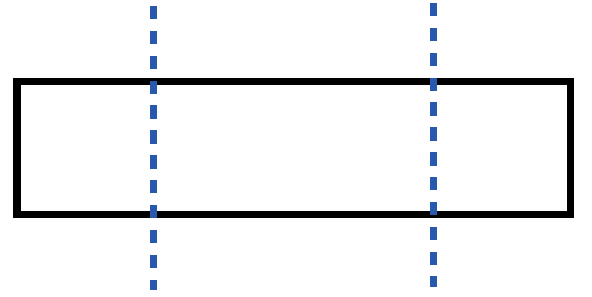
\includegraphics[width=120pt]{kek.pdf}
   \caption{Cake}Example for a visualisation of a cake with two cuts
  	 \end{figure} 
Such an allocation has to be of a special kind, so that the involved players are pleased with the outcome. For the visualisation it is common to use a rectangular cake. The division is performed by parallel cuts. The cake $X$ is represented by the unit interval $X=[0,1] \subseteq \mathbb{R}$. Each subinterval $X'\subseteq X$ or a sequence of disjoint subintervals $$\sideset{}{ }\bigcup\limits_{m\in\mathbb{N}}X'_m$$
with $X'_m\subseteq X$ is called a \emph{portion (or piece)}. The portion of the cake which is received by player $p_i$ is denoted $X_i$. The state is called an \emph{allocation}, when all portions of the cake are owned by players. Each piece has a public size, which can be computed as the sum of all border differences, and the private value of each player, which is constituted by the lower defined valuation function.\\

Every player $p_i\in P_n$ has a \emph{valuation function (valuation)} $v_i:\{X'|X' \subseteq X\} \rightarrow [0,1]\subseteq \mathbb{R}$ with the following properties:
\begin{enumerate}
\item Non-negativity: $v_i(C)\geq 0$ for all $C\subseteq [0,1].$
\item Normalisation: $v_i(\emptyset)=0$ and $v_i([0,1])=1.$
\item Additivity: $v_i(C \cup C')=v_i(C)+v_i(C')$ for disjoint
$C,C'\subseteq [0,1].$\footnote{Monotonicity: If $C' \subseteq C$ then $v_i(C') \leq v_i(C)$. Monotonicity follows from additivity, because for the assumption $C' \subseteq C$ and $A:=C\backslash C'$: $v_i(C)=v_i(A\cup C')=v_i(A)+v_i(C')=\underbrace{v_i(C\backslash C')}_{\geq 0}+v_i(C')\geq v_i(C').$}
\item Divisibility: For all $C\subseteq [0,1]$ and all $\alpha \in
\mathbb{R}$, $0\leq \alpha \leq 1$, there exists a $B\subseteq C$, so that
$v_i(B)=\alpha \cdot v_i(C).$
\item  $v_i$ is continuous: If $0<x<y\leq 1$ with $v_i([0,x])=\alpha$ and
$v_i([0,y])=\beta$, then for every $\gamma \in [\alpha,\beta]$ there exists a $z \in [x,y]$ so that $v_i([0,z])=\gamma.$
\item Non-atomic:  $v_i([x,x])=0$ for all $x\in [0,1].$
\end{enumerate}
%Game theory can be seen as a tool for describing interaction in life's processes. The occurring problems can be simulated by games.  
%Non-cooperated game theory is about single selfish players, and in cooperated the main focus is on forming coalitions. For computer scientists especially the algorithmic game theory is of major interest, because $\dots$. 
\subsection{Concepts in Game Theory}
A brief introduction into the basic concepts of game theory is given and directly applied to the cake-cutting problem. For subsequent applications a probability model is introduced.%The comparison between the classes of games indicate that the best fitting game-theoretic model is the Bayesian game \cite{}. The development of this result and use of the associated solution concepts is described.
 In particular the possible representations of games are in the priority of this chapter. For further reading see \cite{gtt}, \cite{stl} and \cite{ba}. 
\begin{defi}{\textbf{(Game)}}\\
\emph{A \emph{non-cooperative game} $\Gamma=(P_n,S,u)$ consists of the set of players $P_n$, the set of strategies $S$ and the set of utility functions of all players $u$.
\begin{itemize}
\item Each player in the set $P_n=\{p_1,\cdots,p_n\}$ behaves selfish and rational.
\item Each player $p_i$ has his own set of strategies $S_i=\{S_{i,1},S_{i,2}, \ldots\}$. Hereby a \emph{pure strategy} $S_{i,j}$  with $j \in \mathbb{N}$ is a single action.
\item Utility is measuring player's happiness for $p_i$ is $u_i \in \mathbb{R}$.
\end{itemize}}
\end{defi}
Each game has end-states, which are called outcomes. In cake-cutting an outcome is an allocation.
%Definition 2 (Outcome) An outcome is any end-state of the system.
The utility function in cake-cutting is the valuation function. The utility of an allocation for a player is the value of the piece this player obtain in it. From a bigger value follows more happiness for a player.
\begin{defi}{\textbf{(Strategies)}}\\
\emph{ Assume two strategies $S_1$ and $S_2$ for a player $p_1$ and the value $v_1(X_{1,S_1,i})$ and $v_1(X_{1,S_2,i})$ for $i \in \mathbb{N}$ number of possible different allocations.\\
	The strategy $S_1$ \emph{dominates} the strategy $S_2$ if $v_1(X_{1,S_1,i}) \geq v_1(X_{1,S_2,i})$ for all $i$.
		\begin{itemize}
			\item The strategy $S_1$ \emph{strictly dominates} the strategy $S_2$ if $v_1(X_{1,S_1,i}) > v_1(X_{1,S_2,i})$ for all $i$.
			\item The strategy $S_1$ \emph{weakly dominates} the strategy $S_2$ if $v_1(X_{1,S_1,i}) > v_1(X_{1,S_2,i})$ for at least one $i$ and $v_1(X_{1,S_1,i}) \geq v_1(X_{1,S_2,i})$ for all other $i$.
		\end{itemize}
	}\emph{
}\emph{
The strategy $S_1$ is \emph{dominated} by the strategy $S_2$ if $v_1(X_{1,S_1,i}) \leq v_1(X_{1,S_2,i})$ for all $i$.
\begin{itemize}
\item The strategy $S_1$ is \emph{strictly dominated} by the strategy $S_2$ if $v_1(X_{1,S_1,i}) < v_1(X_{1,S_2,i})$ for all $i$.
\item The strategy $S_1$ is \emph{weakly dominated} by the strategy $S_2$ if $v_1(X_{1,S_1,i}) < v_1(X_{1,S_2,i})$ for at least one $i$ and $v_1(X_{1,S_1,i}) \leq v_1(X_{1,S_2,i})$ for all other $i$.
\end{itemize}}
\end{defi}
The strategy $S_1$ can neither dominates nor be dominated in regard to another strategy $S_2$, so $v_1(X_{1,S_1,i}) < v_1(X_{1,S_2,i})$ for at least one $i$ and $v_1(X_{1,S_1,i}) > v_1(X_{1,S_2,i})$ for at least an other $i$. Also  $v_1(X_{1,S_1,i}) = v_1(X_{1,S_2,i})$ for all $i$ is possible, but in this case the strategies can be seen as equal and the player is indifferent between them.\\
%\begin{defi}{\textbf{(Zero-Sum Game / General-Sum Game )}}\\
%\emph{In a \emph{zero-sum game} the sum of the valuations of an allocation is one. Otherwise the game is called %\emph{variable-sum game}.}
%\end{defi}
%Cutting a cake is usually a non-zero-sum game since it allows players to get better off than $\nicefrac{1}{n}$-th. An exception is a cake with equal valuations over the cake.
%\begin{defi}{\textbf{(Repeated Game)}}\\
%\emph{A \emph{repeated game} } 
%\end{defi}
\newline
Another important aspect to consider in studying of games is the amount of information available to the players about past moves of the game or the intentions of his fellow players. 
\begin{defi}{\textbf{(Perfect / Imperfect Information)}}\\
\emph{In a game of \emph{perfect information} every player always knows every move that other players have made before. In a game of \emph{imperfect information} some players sometimes do not know the strategy choices other players have made.}
\end{defi}
\begin{defi}{\textbf{(Incomplete / Complete Information)}}\\
\emph{The games with \emph{incomplete / complete information}, are about the information of the circumstances under which the game is played for example the rules, the order of playing and the set of strategies of the players.}
\end{defi}
\begin{defi}{\textbf{(Mutual / Common Knowledge)}}\\
\emph{An event is \emph{mutual knowledge} if all players know it. \emph{Common knowledge} also requires that all players know the event, all players know that all players know it, and so on ad infinitum.}
\end{defi}
By applying game theory in cutting a cake it is especially important that the valuation functions are private and that no player knows each others private valuation or his own position in the game. Also the players sometimes do not know the moves of other players before them. So cake-cutting is a game with imperfect and incomplete imformation. In game theory for finding solutions in such concepts the unavailable information is imitated through randomness. This also will be done in this work.\\For the further analysis some assumptions have to be made and a probability model to be defined. In cake-cutting the number of different valuation functions over the cake is infinite, so it makes no sense to define the probability for one special valuation. Hence, the possible events in the following chapters depend on special partitions of the cake. The preferences of each player $p_j$ over a partition $X^1, \ldots, X^n$ cutted by a player $p_i$ with $1 \leq i,j \leq n, i \neq j$ can be defined as follows:    
\begin{defi}{\textbf{(Event)}}\\
\emph{An \emph{event} is the selection of a single piece $X^j$ by a player $p_j$ from $X^1, \ldots, X^n$ with $1 \leq j \leq n,\: i \neq j$.}
\end{defi}
\begin{defi}{\textbf{(Probability)}}\\
\emph{For $n$ given disjoint pieces of a cake $X=X^1, \ldots, X^n$ the \emph{probability} for a player $p_j$ to 
choose a piece $X^j$ is given by $${P}(v_j(X^k) \leq v_j(X^n))=\nicefrac{1}{n}$$ for $1 \leq j \leq n,\: j\neq i$ and $1 \leq k < n$} 
\end{defi}
\begin{defi}{\textbf{(Expected Value)}}\\
\emph{The \emph{expected value} for the piece of player $p_i$ is defined by $$\mathbb{E}(v_i(X_i))= \nicefrac{1}{n} \cdot \sum\limits_{k=1}^n v_i(X^k).$$} 
\end{defi}
A game can be rather strategic, where all player move simoultaneous or extensive, where the players move in a fixed or variable order. A game can be represented in normal or in extended form. The normal form is advantageous for games where players move simultaneous, but is not suitable for cake-cutting since it does not respect the order of moves, which is an important part of the following allocation procedures. A better fitting model to represent a cake-cutting game is the extended form as a game tree.
\newpage
\begin{defi}\textbf({Normal Form Game)}\\
\emph{A \emph{normal form game} is a representation of a game in a tabular. In the case for two players the first player chases the row while the second choses the column. Each cell contains a tuple with the values of the obtained pieces, one per player.\begin{itemize}
\item[]The player $p_1$ has two possible strategies $Strategy_a$ and $Strategy_ b$. 
\item[]The player $p_2$ has two possible strategies $Strategy_I$ and $Strategy_ II$.
\item[]If player $p_1$ choose the strategy $Strategy_a$ and player $p_2$ the strategy $Strategy_I$:\\
Player $p_1$ obtains a piece with the value $v_1(X_{1,I,a})$ and player $p_2$ obtains a piece\\with the value $v_2(X_{2,I,a})$
\end{itemize}}
\end{defi}
\begin{table}[htb]
\centering
 \renewcommand{\arraystretch}{1.2} 
\begin{tabular}{c|c|c|}
\cline{2-3}
&\multicolumn{1}{|c|}{$Strategy_a$}& {$Strategy_b$}\\
\hline
\multicolumn{1}{|r|}{$Strategy_I$}&$\left(v_1(X_{1,I,a}), v_2(X_{2,I,a}) \right)$&$\left(v_1(X_{1,I,b}), v_2(X_{2,I,b}) \right)$\\
\hline
\multicolumn{1}{|r|}{$Strategy_{II}$}&$\left(v_1(X_{1,II,a}), v_2(X_{2,II,a}) \right)$&$\left(v_1(X_{1,II,b}), v_2(X_{2,II,b}) \right)$\\
\hline
\end{tabular}
\caption{Game in normal form}\label{Table0}
\end{table}

\begin{defi}\textbf({Extended Form Game)}\\
\emph{An \emph{extended form game} is a tree representation of a game. The tree starts on the left and has the leafs on the right side. The inner nodes are the decision points of the players. The number upon the node is the index of the player whose turn it is.}
\end{defi}
\begin{figure}[h!]
\begin{center}
	\begin{tikzpicture}
		\node[circle,draw,ball color=blue!10,shade=ball,inner sep=5pt] (n1) at (1,5) { };
		\node[circle,draw,ball color=blue!10,shade=ball,inner sep=5pt] (n2) at (5,7) {};
		\node[circle,draw,ball color=blue!10,shade=ball,inner sep=5pt] (n3) at (5,3) {};
		\node[circle,draw,ball color=blue!10,shade=ball,inner sep=5pt] (n4) at (9,8) {};
		\node[circle,draw,ball color=blue!10,shade=ball,inner sep=5pt] (n5) at (9,6) {};
		\node[circle,draw,ball color=blue!10,shade=ball,inner sep=5pt] (n6) at (9,4) {};
		\node[circle,draw,ball color=blue!10,shade=ball,inner sep=5pt] (n7) at (9,2) {};

		\node[draw=none,fill=none] (t1) at (1,5.5) {1};
		\node[draw=none,fill=none] (t2) at (5,7.5) {2};
		\node[draw=none,fill=none] (t1) at (5,3.5) {2};

		\node[draw=none,fill=none,right] at (1.85,6.55) {$Strategy_{I}$};		
		\node[draw=none,fill=none,right] at (1.85,3.5) {$Strategy_{II}$};
		\node[draw=none,fill=none,right] at (6,2.2) {$Strategy_{b}$};
		\node[draw=none,fill=none,right] at (6,3.9) {$Strategy_{a}$};
		\node[draw=none,fill=none,right] at (6,6.2) {$Strategy_{b}$};
		\node[draw=none,fill=none,right] at (6,7.9) {$Strategy_{a}$};
		\node[draw=none,fill=none,right] at (9.5,8) {$\left(v_1(X_{1,I,a}), v_2(X_{2,I,a})\right)$};
		\node[draw=none,fill=none,right] at (9.5,6) {$\left(v_1(X_{1,I,b}), v_2(X_{2,I,b})\right)$};
		\node[draw=none,fill=none,right] at (9.5,4) {$\left(v_1(X_{1,II,a}), v_2(X_{2,II,a}) \right)$};
		\node[draw=none,fill=none,right] at (9.5,2) {$\left(v_1(X_{1,II,b}), v_2(X_{2,II,b}) \right)$};

		\draw (n1) -- (n2);
		\draw (n1) -- (n3);
		\draw (n2) -- (n4);
		\draw (n2) -- (n5);
		\draw (n3) -- (n6);
		\draw (n3) -- (n7);

	\end{tikzpicture}
	\caption{Game in extended form}
\end{center}
\end{figure}
So player $p_1$ choose his strategy first, and then it is player $p_2$'s move. Hereby, only player $p_2$ knows how player $p_1$ moved. The leafs are the end-states of the game with the values the players obtain on the right from them. Around the vertices is the strategy of the acting player. If a path is red it is not good for the first player. If after the obtained values is a lightning the path is not good for the second player.\\
\newline
%%%%%%%%%%%%%%%%%%%%%%%%%%%%%%%%%%%%%%%%%%%%%%%%%%%%%%%%%%%%%%%%%%%%%%%%%%%%%%%%%%%%%%%%%%%%%%%%%%%%%%%%%%%%%%%%
%%%%%%%%%%%%%%%%%%%%%%%%%%%%%%%%%%%%%%%%%%%%%%%%%%%%%%%%%%%%%%%%%%%%%%%%%%%%%%%%%%%%%%%%%%%%%%%%%%%%%%%%%%%%%%%%
%%%%%%%%%%%%%%%%%%%%%%%%%%%%%%%%%%%%%%%%%%%%%%%%%%%%%%%%%%%%%%%%%%%%%%%%%%%%%%%%%%%%%%%%%%%%%%%%%%%%%%%%%%%%%%%%
After some basics it would be interesting to see how game-theory is applicable to cake-cutting. Example \ref{bsp1} illustrates the problem in a game-theoretic manner.
\begin{bsp}
\label{bsp1}
\textcolor{white}{x}\\\\
John Cocke and Tadao Kasami want to divide a chocolate-strawberry-cake. The cake is half chocolate from the left and the right part is strawberry. John Cocke got the first move and is thinking about making three different cuts. After the cuts the two pieces would have the following values:
	\begin{figure}[!h]
		\centering
 		 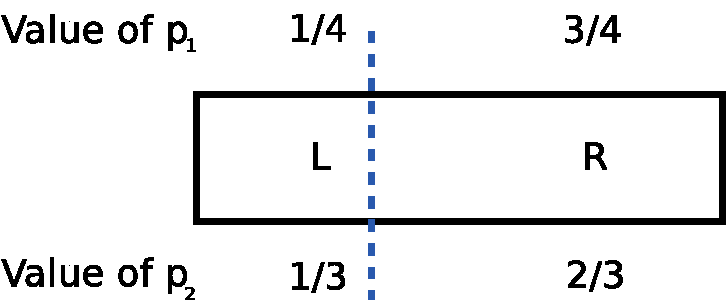
\includegraphics[width=390pt]{bilder/ex1.pdf}
   \caption{C$\&$K cake game}
  	 \end{figure}
  	 \newline
%%%%%%%%%%%%%%%%%%%%%%%%%%%%%%%%%%%%%%%%%%%%%%%%%%%%%%%%%%%%%%%%%%%%%%%%%%%%%%%%%%%%%%%%%%%%%%%%%%%%%%%%%%%%%%
\begin{table}[htb]
\centering
 \renewcommand{\arraystretch}{1.2} 
\begin{tabular}{c|c|c|c|}
\cline{2-4}
&\multicolumn{1}{|c|}{{Leftcut}}& {Middlecut}&{Rightcut}\\
\hline
\multicolumn{1}{|r|}{{L}}&$\left(\nicefrac{3}{4}, ?\right)$&$\left(\nicefrac{1}{2}, ?\right)$&$\left(\nicefrac{2}{5}, ?\right)$\\
\hline
\multicolumn{1}{|r|}{{R}}&$\left(\nicefrac{1}{4}, ?\right)$&$\left(\nicefrac{1}{2}, ?\right)$&$\left(\nicefrac{3}{5}, ?\right)$\\
\hline
\end{tabular}
\caption{C$\&$K cake game in normal form}\label{Table1}
\end{table}
Before doing so, he analyses his situation via the normal form:\\Since the valuation is a private function, he does not know the preferences of his colleague and has to assume that Tadao is indifferent between the two pieces. %By choosing not the middlecut he has the possibility to get more than a half, but also to make a loss.
Tadao is waiting for John's move and will choose his best strategy in the extended game form: 
%%%%%%%%%%%%%%%%%%%%%%%%%%%%%%%%%%%%%%%%%%%%%%%%%%%%%%%%%%%%%%%%%%%%%%%%%%%%%%%%%%%%%%%%%%%%%%%%%%%%%%%%%%%%%%
\begin{figure}[h!]
\begin{center}
	\begin{tikzpicture}
		\node[circle,draw,ball color=blue!10,shade=ball,inner sep=5pt] (n1) at (1,5) { };
		\node[circle,draw,ball color=blue!10,shade=ball,inner sep=5pt] (n2) at (5,3) {};
		\node[circle,draw,ball color=blue!10,shade=ball,inner sep=5pt] (n3) at (5,5) {};
		\node[circle,draw,ball color=blue!10,shade=ball,inner sep=5pt] (n4) at (5,7) {};
		\node[circle,draw,ball color=blue!10,shade=ball,inner sep=5pt] (n5) at (9,5.5) {};
		\node[circle,draw,ball color=blue!10,shade=ball,inner sep=5pt] (n6) at (9,4.5) {};
		\node[circle,draw,ball color=blue!10,shade=ball,inner sep=5pt] (n7) at (9,7.5) {};
		\node[circle,draw,ball color=blue!10,shade=ball,inner sep=5pt] (n8) at (9,6.5) {};
		\node[circle,draw,ball color=blue!10,shade=ball,inner sep=5pt] (n9) at (9,3.5) {};
		\node[circle,draw,ball color=blue!10,shade=ball,inner sep=5pt] (n10) at (9,2.5) {};

		\node[draw=none,fill=none] (t1) at (1,5.5) {1};
		\node[draw=none,fill=none] (t2) at (5,7.5) {2};
		\node[draw=none,fill=none] (t1) at (5,3.5) {2};
		\node[draw=none,fill=none] (t1) at (5,5.5) {2};

		\node[draw=none,fill=none,right] at (1.85,6.35) {Leftcut};
		\node[draw=none,fill=none,right] at (1.85,5.25) {Middlecut};
		\node[draw=none,fill=none,right] at (1.85,3.65) {Rightcut};
		\node[draw=none,fill=none,right] at (7,2.53) {R};
		\node[draw=none,fill=none,right] at (7,3.49) {L};
		\node[draw=none,fill=none,right] at (7,4.53) {R};
		\node[draw=none,fill=none,right] at (7,5.49) {L};
		\node[draw=none,fill=none,right] at (7,6.53) {R};
		\node[draw=none,fill=none,right] at (7,7.49) {L};
		\node[draw=none,fill=none,right] at (9.5,7.5) {$\left(\nicefrac{3}{4}, \nicefrac{1}{3}\right)$};
		\node[draw=none,fill=none,right] at (9.5,6.5) {$\left(\nicefrac{1}{4}, \nicefrac{2}{3}\right)$};
		\node[draw=none,fill=none,right] at (9.5,5.5) {$\left(\nicefrac{1}{2}, \nicefrac{3}{7}\right)$};
		\node[draw=none,fill=none,right] at (9.5,4.5) {$\left(\nicefrac{1}{2}, \nicefrac{4}{7}\right)$};
		\node[draw=none,fill=none,right] at (9.5,3.5) {$\left(\nicefrac{2}{5}, 1\right)$};
		\node[draw=none,fill=none,right] at (9.5,2.5) {$\left(\nicefrac{3}{5}, 0\right)$};
		
		
		\draw (n1) -- (n2);
		\draw (n1) -- (n3);
		\draw (n1) -- (n4);
		\draw (n3) -- (n5);
		\draw (n3) -- (n6);
		\draw (n4) -- (n7);
		\draw (n4) -- (n8);
		\draw (n2) -- (n9);
		\draw (n2) -- (n10);

	\end{tikzpicture}
	\caption{C$\&$K cake game in extended form}
\end{center}
\end{figure}
\newline For John the graph shows that if he stays secure he would obtain $v_1(X_1)=\nicefrac{1}{2}$. Otherwise he would get $\nicefrac{1}{4}$ or $\nicefrac{2}{5}$. So to make the middlecut is his best possible move.
\end{bsp}
%%%%%%%%%%%%%%%%%%%%%%%%%%%%%%%%%%%%%%%%%%%%%%%%%%%%%%%%%%%%%%%%%%%%%%%%%%%%%%%%%%%%%%%%%%%%%%%%%%%%%%%%%%%%%%%%
%%%%%%%%%%%%%%%%%%%%%%%%%%%%%%%%%%%%%%%%%%%%%%%%%%%%%%%%%%%%%%%%%%%%%%%%%%%%%%%%%%%%%%%%%%%%%%%%%%%%%%%%%%%%%%%%
%%%%%%%%%%%%%%%%%%%%%%%%%%%%%%%%%%%%%%%%%%%%%%%%%%%%%%%%%%%%%%%%%%%%%%%%%%%%%%%%%%%%%%%%%%%%%%%%%%%%%%%%%%%%%%%%
\subsection{Different Types of Fairness}
As indicated by the name, fairness plays an important role in fair division. But how is fairness defined? It can be seen as a valuation criterion of an allocation, which can be normalized and gives a possibility to compare different allocations. Usually the fairness criteria are distinguished between the following:
\begin{defi}{\textbf{(Proportional or Simple Fair)}}
\newline \emph{An allocation is \emph{proportional (simple fair)} if
$v_i(X_i) \geq \nicefrac{1}{n}$ for each player $p_i \in P_n$.}
\end{defi}
\begin{defi}{\textbf{(Envy-Freeness)}}
\newline \emph{An allocation is \emph{envy-free} if $v_i(X_i) \geq
v_i(X_j)$ for each couple of players $p_i, p_j \in P_n$.}
\end{defi}
\vsp
%\begin{defi}{\textbf{(Equity)}}
%\newline An allocation is \emph{equitable}, if $v_i(X_i) =
%\alpha$ for each player $p_i \in P_n$ and $0 \leq \alpha \leq 1$ \footnote{ If $\alpha = 1/n$ the allocation is called \emph{exact}.}.
%\end{defi}
%

Theorem \ref{first_theorem} shows the correlation between the two types of fairness.
%
\begin{lem}
\label{first_theorem}
\textcolor{white}{x}
\begin{enumerate}
\item Every envy-free allocation is proportional.
\item An allocation between two players is envy-free if and only if it is proportional.
\end{enumerate}
\end{lem}
\begin{proof}
\textcolor{white}{x}
\begin{enumerate}
\item Proof by contradiction:\\ Assume $A$ is an envy-free allocation, but not proportional. From envy-freeness follows $v_i(X_i) \geq v_i(X_j)$ for each pair of players $p_i, p_j \in P_n$ and so each player has at least an as much valuable piece of cake as each other player in his own valuation. Hereby each player owns in his own valuation at least as much as each of the $(n-1)$ other players. The smallest value for which it is possible that $(n-1)$ players and the considered players own the same value in the valuation of the considered player is $\nicefrac{1}{((n-1)+1)}$. Each player owns in his valuation at least $\nicefrac{1}{n}$. \blitza The allocation $A$ is proportional. %$\lightning$ 
\\Therefore, all envy-free allocations are proportional.
\item ''$\Leftarrow$'' For two players $p_1$ and $p_2$ an allocation is proportional if each player has $p_i(X_i) \geq \nicefrac{1}{2}$ for $i \in \{1,2\}$. The whole cake has the value $v_i(X)=1$ for $i \in \{1,2\}$. And so for each player $v_i(X-X_i) \leq 1- \nicefrac{1}{2} = \nicefrac{1}{2}$  for $i \in \{1,2\}$. The value of the piece not obtained by a player is smaller or equal to his obtained piece. So the player $p_1$ does not envy the other player $p_2$ and vice versa.\\ ''$\Rightarrow$'' Follows from part 1.\\
\end{enumerate}
\end{proof}
A different criterion to valuate the quality of an allocation is efficiency. Further correlations between the fairness criteria and efficiency can be found in \cite{eff}. 
\begin{defi}{\textbf{(Efficiency)}}
\newline \emph{An allocation \[A=\{X_1,\dots, X_n\}\] is \emph{efficient (Pareto optimal)} if there is no other allocation \[A'=\{X'_1,\dots, X'_n\}\] such that \[v_i(X_i)\leq v_i(X'_i)\] for all players $p_i \in P_n$ and for at least one player the inequality is strict.}
\end{defi}
%
\begin{lem}
\label{theorem2}
\textcolor{white}{x}
	\begin{enumerate}
		\item Envy-freeness and proportionality do not imply efficiency.
		\item Efficiency does not imply proportionality and so envy-freeness.
	\end{enumerate}
\end{lem}

\begin{proof}
\textcolor{white}{x}
	\begin{enumerate}
\item Imagine the following allocation with three players. Each player's portion can consist up to three pieces. The value of the whole portion is (because of the additivity of the valuation) the sum of the pieces :
		\begin{table}[htb]
		\centering
		\renewcommand{\arraystretch}{1.2}
		\begin{tabular}{c|cc}
		& $X_1 =X_1'\cup X_1''$& $X_2 =X_2'\cup X_2''$\\
		\hline
		\multirow{2}*{$p_1$} & \multirow{2}*{\textcolor{blue}{$\nicefrac{1}{2}=\nicefrac{1}{3}+\nicefrac{1}{6}$}} & \multirow{2}*{$\nicefrac{1}{2}=\nicefrac{1}{12}+\nicefrac{11}{12}$}\\ \\
  \multirow{2}*{$p_2$} & \multirow{2}*{$\nicefrac{1}{3}=\nicefrac{1}{6}+\nicefrac{1}{6}$} & \multirow{2}*{\textcolor{blue}{$\nicefrac{2}{3}=\nicefrac{2}{3}+0$}} \\\\
 		\end{tabular}	 
\caption{Example for envy-freeness does not imply efficiency}\label{Table3}
\end{table}
\newline This allocation is obviously envy-free, since $v_1(X_1) = v_1(X_2)$ and $v_2(X_2) > v_2(X_1)$. It is not efficient, because if the player $p_1$ would get $p_2$'s portion $X_2''$, $p_1$ would get a more valuable piece of the cake and $p_2$ would not get a less valuable piece. Since in Theorem 1 was shown that envy-freeness implies proportionality, this example also demonstates that proportionality does not imply efficiency.
		\item Allocating the whole cake to one player is efficient, but definitely not proportional and therefore not envy-free.
	\end{enumerate}
\end{proof}
In \cite{brams2} the authors show a general argument that no finite bounded protocol can exist for such an allocation that is both proportional and efficient at the same time.
%%%%%%%%%%%%%%%%%%%%%%%%%%%%%%%%%%%%%%%%%%%%%%%%%%%%%%%%%%%%%%%%%%%%%%%%%%%%%%%%%%%%%%%%%%%%%%%%%%%%%%%%%%%%%%%%
%%%%%%%%%%%%%%%%%%%%%%%%%%%%%%%%%%%%%%%%%%%%%%%%%%%%%%%%%%%%%%%%%%%%%%%%%%%%%%%%%%%%%%%%%%%%%%%%%%%%%%%%%%%%%%%%
%%%%%%%%%%%%%%%%%%%%%%%%%%%%%%%%%%%%%%%%%%%%%%%%%%%%%%%%%%%%%%%%%%%%%%%%%%%%%%%%%%%%%%%%%%%%%%%%%%%%%%%%%%%%%%%%
\subsection{Different Types of Protocols}
It is very important to understand the types, structure and design of protocols, which are analysed in this work.\\
\newline
Informal: (Algorithm)
\newline An \emph{algorithm} is an effective method for solving a problem, which is composed of a finite sequence of instructions.
\begin{defi}{\textbf{(Cake-Cutting-Protocol)}}
\newline \emph{A \emph{cake-cutting-protocol} (protocol for short) is an algorithm with a fixed number of players and the following properties:
\begin{itemize}
\item{A protocol consists of rules and strategies.\\ \emph{Rules} are requirements, which \emph{have to} be followed by the players. Furthermore, it is possible to ensure that the players obey the rules.\\	
%
\emph{Strategies} are recommendations, which \emph{can} be followed for getting the guaranteed fair share. It  is impossible to verify whether a player follows the strategy of the protocol.}
\item Each player should be able to cut the cake at a specific moment independent of other players.
\item The protocol has no information about the valuation of the players, except of those it got from the steps before.
\end{itemize}}
\end{defi}
\textbf{Comment:} Only such protocols are interesting where the actions of one player does not harm the other players.
\begin{defi}{\textbf{(Proportional/ Envy-Free Protocol)}}\\
\emph{A cake-cutting \emph{protocol} is called \emph{proportional} or \emph{envy-free} if independent of the players' valuations, each allocation is proportional or envy-free provided that all players follow the rules and strategies given by the protocol.}
\end{defi}
The development of such protocols is one of the main goals of cake-cutting \cite{robertson:cake-cutting}.

\begin{defi}{\textbf{(Finite (Discrete) / Continuous (Moving-Knife) Protocol)}}
\newline \emph{A \emph{finite (discrete) protocol} gives a solution after a finite number of queries (valuations, marks, $\ldots$). In a \emph{continuous (moving-knife) protocol} a player has to make up to infinitely many queries.}
\end{defi}
\begin{defi}{\textbf{(Finite Bounded / Finite Unbounded Protocol))}}
\newline \emph{A \emph{finite bounded protocol} has an upper bound of steps for all possible valuations. The number of those steps is correlated with the number of players only in some cases. A \emph{finite unbounded protocol} has no approximated number of steps.}
\end{defi}
The most desirable protocols are the finite bounded because of the ease of their implementation. \\
In the last sixty years the number of proportional finite bounded protocols has grown for an arbitrary number of players. But still no envy-free finite bounded protocol for an arbitrary $n$ is known \cite{chen:truth}. Only for three or less players a cake can be divided in a fixed number of steps, so that it is envy-free. For this reason, only proportional protocols are considered in the further work.
%%%%%%%%%%%%%%%%%%%%%%%%%%%%%%%%%%%%%%%%%%%%%%%%%%%%%%%%%%%%%%%%%%%%%%%%%%%%%%%%%%%%%%%%%%%%%%%%%%%%%%%%%%%%%%%%
%%%%%%%%%%%%%%%%%%%%%%%%%%%%%%%%%%%%%%%%%%%%%%%%%%%%%%%%%%%%%%%%%%%%%%%%%%%%%%%%%%%%%%%%%%%%%%%%%%%%%%%%%%%%%%%%
%%%%%%%%%%%%%%%%%%%%%%%%%%%%%%%%%%%%%%%%%%%%%%%%%%%%%%%%%%%%%%%%%%%%%%%%%%%%%%%%%%%%%%%%%%%%%%%%%%%%%%%%%%%%%%%%
%\newpage
\section{Strategyproofness}
\label{sven_hat_recht}
In the scope of this work it is assumed that players are selfish and try to increase the value of their portion. In order to do so, they may misrepresent their valuation on the cake. The goal is to prevent this.
It is assumed that a set of players and the divisible ressource are given. Each player knows his preferences, but has not valued the ressource yet. The protocol shows the cake or parts of it to a certain player and requires from him to follow the rules, so to make a mark or a cut, or to choose at least one piece of the cake. The protocol also makes a recommendation to the player by using a strategy. The player can deside whether to follow it or to made up an other strategy.
\begin{defi}{\textbf{(Non-Truthful (Cheating) / Honest Player)}}\\
\emph{Every strategy is called \emph{non-truthful} except of the strategy recommended by the protocol. A player who follows a non-truthful strategy will be called a \emph{non-truthful (cheating) player}. Otherwise the player is called \emph{honest}.}
\end{defi}
\begin{defi}{\textbf{(True Value Function)}}\\
\emph{A \emph{true value function} provides the value of the piece a player would receive by following the recommended strategy. This value is at least proportional in a proportional protocol.}
\end{defi}
A strategy $S_{1}$ is better for player $p_{i}$ than another strategy $S_{2}$ if the value of the obtained piece by following $S_{1}$ is bigger than by following $S_{2}$.
\begin{defi}{\textbf{(Risk Aversion \cite{brams})}}\\
\emph{A player is \emph{risk averse} if he will never choose a strategy that may yield a more valuable piece of cake if it entails the possibility of getting less than a piece of a guaranteed size.}
\end{defi}
\begin{defi}{\textbf{\\(Strategyproofness of a Proportional Protocol \cite{lindner:degrees})}}\\
\emph{A proportional cake-cutting protocol is said to be \emph{strategyproof for risk averse players} (SPP for short) if a cheating player is no longer guaranteed a proportional share, whereas all other players (provided they play truthful) are still guaranteed to receive their proportional share.}
\end{defi}
%\textbf{Notice:} The actions of a player do not harm any of the other players.
%\begin{defi}{\textbf{(Truthful Allocation)}}
%An allocation is \emph{truthful} if the value of the cake obtained by a player by reporting false is not greater than by reporting the truth.
%\end{defi}

\begin{defi}{\textbf{(Strategyproofness in the sense of \cite{pie})}}\\
\label{blub}
\emph{A protocol is \emph{strategyproof} if no player has a strategy that is assuredly better than his true value function.}
\end{defi}
The strategyproofness in the sense of Definition \ref{blub} will be called weak strategyproofness (WSP for short) since it is always true for a proportional protocol, see also \cite{ccc}.
\begin{bsp}
\label{bsp222}
\textcolor{white}{x}\\\\
Assume the case when all valuations over the cake are equal, and all players, except of the cheating one follow the strategy provided by the protocol. Each of the honest players will get his proportional share, because the protocol is proved to be proportional. The cheating player also values those pieces as $\nicefrac{1}{n}$ or more. Sharing a cake with $(n-1)$ other players means for the cheater that $\nicefrac{(n-1)}{n}$ or a more valuable part of the cake is allocated to other players and so only the value of $\nicefrac{1}{n}$ or less remains for him independent of his strategy. He would never obtain more than a proportional piece.
\end{bsp}
%This characteristic is not significant, since valuations like in Example \ref{bsp222} of the players where the %cheater would never get more than a proportional piece exist always.\\
%
%Due to the fact that valuations like in Example \ref{bsp222} do always exist, a cheating player 
%
%A controversial point is that with this definition a player with a non-truthful strategy which obtains in one %special case the same valuable piece, like the true value function and in all other strictly more valuable %pieces would stay honest.\\
As depicted in Example \ref{bsp222}, there always exists a valuation such that in an allocation a cheating player will never obtain more than a proportional piece. Hence, weak strategyproofness is not significant.
\newline
A stronger condition comes from the social choice literature:

\begin{defi}{\textbf{(Strategyproofness in the sense of \cite{why})}}\\
\label{laberlaberlaber}
\emph{A protocol is \emph{strategyproof} if the true value function dominates every other strategy.}
\end{defi}

%Assume the statement is true, where each player acts truthful by following his best strategy, which yields to a maximum possible allocation for a player ''$\Leftrightarrow$'' Nash-equilibrium. But there is a problem, like \cite{malik} detected no known algorithm can fulfill this promise. The appealing alternative is the guarantee of a fair share for telling the truth.\\
In order to prevent misunderstandings, in this work strategyproofness in the sense of Definition \ref{laberlaberlaber} will be called strong strategyproofness (SSP for short). It can be shown that none of the known cake-cutting protocols is able to fulfill the strong strategyproofness criteria, if the valuation of the players is not equal. All protocols shown in Chapter \ref{sven_hat_recht} work for two players in exactly the same way as Cut $\&$ Choose. Example \ref{bsp3} is similar to the one in \cite{chen:truth}.

\begin{bsp}
\label{bsp3}
\textcolor{white}{x}\\\\
John Warner Backus and Peter Naur are celebrating and Donald E. Knuth has brought a huge marzipan cake with an enormous cherry on the left side. John loves cherries and hates marzipan, and Peter is just very hungry. The pioneers of computer science apply Cut $\&$ Choose (see Chapter \ref{cuc}). Peter is the cutter, and his best strategy would be to separate the cake from the cherry. If Peter had full knowledge (which would not violate the preconditions of strategyproofness in \cite{why}) about the valuations of John, he would benefit from cheating. From Table \ref{Table4} he would know, that John would always take the left piece and so he could easily maximize the value of his portion. Hence, this algorithm is not strongly strategyproof.  
\end{bsp}
\begin{table}[htb]
\centering
 \renewcommand{\arraystretch}{1.2} 
\begin{tabular}{c|c|c|}
\cline{2-3}
&\multicolumn{1}{|c|}{{Only Cherry}}& {Middlecut}\\
\hline
\multicolumn{1}{|r|}{{L}}&$\left(\nicefrac{9}{10}, 1\right)$&$\left(\nicefrac{1}{2}, 1\right)$\\
\hline
\multicolumn{1}{|r|}{{R}}&$\left(\nicefrac{1}{10}, 0\right)$&$\left(\nicefrac{1}{2}, 0\right)$\\
\hline
\end{tabular}
\caption{B$\&$N cake game in normal form}\label{Table4}
\end{table}
In strong strategyproofness a player would never get a more valuable piece by lying independent of the valuation of the other players.\\
\newline
After a counterexample in \cite{ccc} the definition of strategyproofness in \cite{pie} was restricted to the case with non-equal valuations and for the general case changed to:

\begin{defi}{\textbf{(Strategyproofness in the sense of \cite{note})}}\\
\emph{A protocol is \emph{strategyproof} (SP for short) if no player has a strategy that is at least as well and sometimes better than his true value function.}
\end{defi}
%The question arises whether a protocol can enforce truthfulness.\\
%An example will be the following case where $n$ players cut the cake in pieces with $v_i(X_i)=\nicefrac{1}{n}$ and then allocate them randomly to the players.\\
Imagine a non-truthful strategy with one allocation where the cheating player would obtain a bit less valuable piece than by the recommended strategy and one thousand other possible allocations this player would get the whole cake, while in the recommended strategy he would get just his proportional share. By the upper defnitions this player would stay honest, but which selfish and rational player would really do this?\\
A possibility to handle those situations gives a game-theoretical approach in the following definition:
\begin{defi}{\textbf{(Game-Theoretic Strategyproofness)}}\\
\emph{A protocol is \emph{game-theoretic strategyproof} (GTSP for short) if no player has a strategy with a higher expected value than the expected value of his true value function.}
\end{defi}
\subsection{Correlation between Strategyproofness Criteria}
\begin{lem}
\label{thm5} The relation between different strategyproofness criteria is the following:
%If the criteria is not fulfilled then $$notWPP \Rightarrow^{5} notSP \Rightarrow^{6} notSP \Rightarrow^{7} notSPP$$ and
%$$notSP \Rightarrow^{8} notGTSP$$
\begin{figure}[h!]
\begin{center}
	\begin{tikzpicture}
		
		\node[draw=none,fill=none] (n1) at (1,5) {$SPP$};
		\node[draw=none,fill=none] (n2) at (2.5,5) {$SP$};
		\node[draw=none,fill=none] (n3) at (4,5) {$WSP$};
		\node[draw=none,fill=none] (n4) at (2.5,4) {$GTSP$};
		\node[draw=none,fill=none] at (1.87,5.14) {$\impl{1}$};
		\node[draw=none,fill=none] at (3.2, 5.14) {$\impl{2}$};
		\node[rotate=90, left] at (2.36, 5.03) {$\impl{\textcolor{white}{3}}$};
		\node[draw=none,fill=none] at (2.25, 4.43) {\scalebox{0.72}{$3$}};
	\end{tikzpicture}
\end{center} 
\end{figure}
\end{lem}
\begin{proof}
\textcolor{white}{x}
\begin{enumerate}
\item If a protocol is $SPP$, then for every player in each strategy except of the recommended one exists at least one allocation $A_c$. In $A_c$ the cheating player $p_c$ receives a piece $X_c$ which is not proportional. Since in a proportional protocol all allocations guarantee a proportional share to every player, the value of his piece $X_c$ is less than he would obtain by following the recommended strategy. So the protocol is $SP$.   
%Es gibt keine Strategie mit alle Fälle mindestens proportional(Bei jeder strategie gibt es einen Fall mit weniger als proportional) \\
\item If a protocol is $SP$, then for every player in each strategy except of the recommended one exists at least one allocation $A_c$. In $A_c$ the cheating player $p_c$ receives a piece $X_{c}$ instead of $X_{\neg c}$, which he had received by following the recommended strategy. The value of $X_c$ is smaller or equal to the value of $X_{\neg c}$. So no non-truthful strategy exist where the cheating player gets in all allocations a more valuable piece than in the recommended one. The protocol is $WSP$.
\pagebreak
%SP-Es gibt keine Strategie mit alle Fälle mindestens einmal mehr und keinmal weniger als TRUE(proportional oder mehr)(Bei jeder strategie gibt es einen Fall mit weniger oder keinen mit mehr als TRUE(proportional oder meh))\\
\item \textbf{Proof by contradiction:}\\
\newline
Assumption: If a protocol is $notSP$ then it is not $notGTSP$.\\
If a protocol is $notSP$, then there is one player with a strategy, which is not the recommended one. And for all allocations $A_{S_c}$ the cheating player $p_c$ receives a piece $X_{S_c}$ instead of $X_{S_{\neg c}}$, which he had received by following the recommended strategy. The value of $X_{S_c}$ is at least equal to the value of $X_{S_{\neg c}}$. In one allocation $A_{S'_c}$ the value of $X_{S'_c}$ is bigger than the value of $X_{S'_{\neg c}}$. Let $r$ be the number of all possible allocations. The expected value of the strategy ${S_c}$ at least equal with the expected value of the recommended strategy for the $r-1$ allocations since the expected value for the received pieces $X_{S_c}$ is at least equal to the expected value for the pieces $X_{S_{\neg c}}$. The expected value for the piece $X_{S'_c}$ is bigger than the expected value for $X_{S'_{\neg c}}$. The general expected value is $\mathbb{E}(S_c)>\mathbb{E}(S_{\neg c})$ and is particularly not $\mathbb{E}(S_c)\leq \mathbb{E}(S_{\neg c})$.\blitza So the protocol is $notGTSP$.  
\newline
So $notSP \Rightarrow notGTSP$ and therefore $GTSP \Rightarrow SP$.
%WSP-Es gibt keine Strategie mit alle Fälle mindestens mehr oder gleich TRUE(proportional oder mehr)(Bei jeder strategie gibt es einen Fall mit weniger oder gleich TRUE(proportional  oder mehr))\\
\end{enumerate}
\end{proof} 
\begin{lem} The relation between different strategyproofness criteria is the following:
\begin{figure}[h!]
\begin{center}
	\begin{tikzpicture}
		
		\node[draw=none,fill=none] (n1) at (1,5) {$SPP$};
		\node[draw=none,fill=none] (n2) at (2.5,5) {$SP$};
		\node[draw=none,fill=none] (n3) at (4,5) {$WSP$};
		\node[draw=none,fill=none] (n4) at (2.5,4) {$GTSP$};
		\node[draw=none,fill=none] at (1.87,5.14) {$\notimplleft{1}$};
		\node[draw=none,fill=none] at (3.2, 5.14) {$\notimplleft{2}$};
		\node[rotate=90, left] at (2.36, 4.83) {$\notimplleft{\textcolor{white}{3}}$};
		\node[draw=none,fill=none] at (2.2, 4.62) {\scalebox{0.72}{3}};
	\end{tikzpicture}
\end{center} 
\end{figure}
\end{lem}
\begin{proof}
\textcolor{white}{x}\\
\newline
Assume three different protocols for two players $p_1$ and $p_2$. All of them have two possible allocations $A_1$ and $A_2$, which have the same probability. In the first protocol and in the third protocol by using the recommended strategy $S_\neg c$ and the non-truthful strategy $S_c$ the player $p_2$ gets the same values in $A_1$ and $A_2$. In the second protocol he obtains strictly more by using the non-truthful strategy $S_c$  than the recommended strategy $S_\neg c$ in $A_1$ and in $A_2$.The values of $p_1$ are shown in the four tables below:\\
\begin{table}[htb]
		\centering
		\renewcommand{\arraystretch}{1.2}
		\begin{tabular}{cc}
		\multicolumn{2}{c}{
		\begin{tabular}{c|cc}
		& in $A_1$& in $A_2$\\
		\hline
		$p_1(X_1)$ by $S_\neg c$ & {$\nicefrac{1}{2}$} & $\nicefrac{2}{3}$\\ 
  $p_1(X_1)$ by $S_c$& $\nicefrac{1}{2}$ & {$\nicefrac{1}{2}$}\\ 
 		\end{tabular}}	 \\	
 		&\\ 
\multicolumn{2}{c}{Protocol 1: $SPP \not\Leftarrow SP$}\\
\begin{tabular}{c|cc}
		& in $A_1$& in $A_2$\\
		\hline
		$p_1(X_1)$ by $S_\neg c$ & {$\nicefrac{7}{8}$} & $\nicefrac{3}{4}$\\ 
  $p_1(X_1)$ by $S_c$& $1$ & {$\nicefrac{3}{4}$}\\ 
 		\end{tabular}&\begin{tabular}{c|cc}
		& in $A_1$& in $A_2$\\
		\hline
		$p_1(X_1)$ by $S_\neg c$ & {$\nicefrac{1}{2}$} & $\nicefrac{4}{7}$\\ 
  $p_1(X_1)$ by $S_c$& $1$ & {$\nicefrac{3}{7}$}\\ 
 		\end{tabular}\\	 
 		&\\
Protocol 2: $WSP \not\Leftarrow SP$& Protocol 3: $GTSP \not\Leftarrow SP$
\end{tabular}
\caption{Counter-examples for the correlation between the strategyproofness criteria}\label{234}
\end{table}

\begin{enumerate}
\item[1] $SPP \not\Leftarrow SP$\\
By following the non-truthful strategy $S_c$ the player $p_1$ gets always $p_1(X_1)=\nicefrac{1}{2}$. In the allocation $A_2$ he obtains less by following the non-truthful strategy $S_c$ in particular $\nicefrac{1}{2} < \nicefrac{2}{3}$. With that outcome the player $p_1$ would stay honest and this protocol is $SP$. But $\nicefrac{1}{2}$ is proportional so the protocol is $notSPP$. 
\item[2] $SP \not\Leftarrow WSP$\\
By following the non-truthful strategy $S_c$ and the recommended strategy $S_{\neg c}$ the player obtains the same value in the allocation $A_2$: $\nicefrac{3}{4} = \nicefrac{3}{4}$. So the player $p_1$ has not got a more valuable piece and so he would stay honest and this protocol is $WSP$. But the value by following the non-truthful strategy $S_c$ is bigger in his own valuation because $1 > \nicefrac{7}{8}$ in $A_1$. In the other allocation $A_2$ the obtained values are equal. So the player $p_1$ has a more valuable piece in one allocation and the same value in the other so the protocol is $notSP$.
\item[3] $GTSP \not\Leftarrow SP$\\
Since in the allocation $A_2$ by following the non-truthful strategy $S_c$ the player $p_1$ get $\nicefrac{3}{7}$ smaller than $\nicefrac{4}{7}$ by following the recommended strategy $S_{\neg c}$. He would stay honest and this protocol is $SP$. But the expected value for the recommended strategy is $\nicefrac{(\nicefrac{1}{2}+\nicefrac{4}{7})}{2}=\nicefrac{15}{28}$, which is smaller than $\nicefrac{(1+\nicefrac{3}{7})}{2}=\nicefrac{20}{28}$. So the protocol is $notGTSP$. 
\end{enumerate}
\end{proof}

\pagebreak
%There are two independent types of strategyproofness to show for having a complete quantity of results. The start will be from the left side until one of the criteria is fulfilled, then the other strategyproofness further on the right follow from Theorem \ref{thm5}. Independently a proof for the game-theoretic strategyproofness has to be given, since it cannot be followed from the other. 
\subsection{The Cut $\&$ Choose Protocol}
\label{cuc}
Representation is inspired by \cite{Barbanel}
\begin{table}[htb]
\begin{tabular*}{\textwidth}[]{|@{\extracolsep{\fill}}l|l|c|}
\hline
\hline
\multicolumn{3}{|c|}{\textbf{Cut $\&$ Choose for $n=2$}}\\
\hline
\multicolumn{1}{|c|}{\textbf{Rules}}& \textbf{Player $p_1$ strategy}& \multicolumn{1}{c|}{\textbf{Player $p_2$ strategy}}\\
\hline
$\:$1. Player $p_1$ partitions the cake $X$ &Partition $X$ into two&\\
$\:\:\:\:\:\:\:$into two pieces $\{X',X-X'\}$&pieces of equal value&\\
\hline
$\:$2. Player $p_2$ chooses one piece&&Choose the bigger value\\
\hline
$\:$3. Player $p_1$ gets the remaining&&\\
$\:\:\:\:\:\:\:$piece&&\\
\hline
\end{tabular*}
\caption{Cut $\&$ Choose rules and strategies}\label{cc}
\end{table}
\begin{lem}
\label{thm7}
Cut $\&$ Choose is game-theoretic strategyproof.
\end{lem}
\begin{proof}
\textcolor{white}{x}\\\\
\textbf{Options for not following the recommended strategy:}
\begin{itemize}
\item Player $p_2$ takes the less valuable piece. This can not be his intention, because then he has a piece with less value.
\item Player $p_1$ cuts the cake into two unequal pieces. The chance to get less in his valuation is equal to the chance to get more in his valuation of the cake. In stochastic terms it means, that the expected value at the end of the allocation will be in the honest case: $$ \mathbb{E}(v_1(X_1))=P(v_2(X')\leq v_2(X-X'))\cdot v_1(X')+P(v_2(X')\leq v_2(X'))\cdot v_1(X-X')$$$$=\nicefrac{1}{2} \cdot \nicefrac{1}{2}+\nicefrac{1}{2} \cdot \nicefrac{1}{2}=\nicefrac{1}{2} $$ and in the dishonest case: $$ \mathbb{E}(v_1(X_1))=P(v_2(X')\leq v_2(X-X'))\cdot v_1(X')+P(v_2(X-X')\leq v_2(X'))\cdot v_1(X-X')$$$$=\nicefrac{1}{2} \cdot v_1(X') +\nicefrac{1}{2} \cdot v_1(X-X') =\nicefrac{1}{2} \cdot \underbrace{v_1(X)}_{=1}=\nicefrac{1}{2}$$ According to the definition of game-theoretical strategyproofness in the case with equal expected values the player would stay honest. Cut $\&$ Choose is game-theoretical strategyproof.
\end{itemize}
\end{proof}
\pagebreak
\begin{lem}
\label{thm6}
Cut $\&$ Choose is strategyproof for proportional protocols.
\end{lem}
\begin{proof}
\textcolor{white}{x}\\\\
For the proof a general presentation of Cut $\&$ Choose game in extended form is used. W. l. o. g. the non-truthful cut is performed on the right part of the cake. The variables have the following restrictions: $$0 \leq a \leq 1,\: 0 < \epsilon \leq \nicefrac{1}{2},\: 0 \leq \delta \leq 1\tiny{-}a$$
\begin{figure}[h!]
\begin{center}
	\begin{tikzpicture}
		\node[circle,draw,ball color=red!20,shade=ball,inner sep=5pt] (n1) at (1,5) { };
		\node[circle,draw,ball color=blue!10,shade=ball,inner sep=5pt] (n2) at (5,7) {};
		\node[circle,draw,ball color=red!20,shade=ball,inner sep=5pt] (n3) at (5,3) {};
		\node[circle,draw,ball color=blue!10,shade=ball,inner sep=5pt] (n4) at (9,8) {};
		\node[circle,draw,ball color=blue!10,shade=ball,inner sep=5pt] (n5) at (9,6) {};
		\node[circle,draw,ball color=blue!10,shade=ball,inner sep=5pt] (n6) at (9,4) {};
		\node[circle,draw,ball color=red!20,shade=ball,inner sep=5pt] (n7) at (9,2) {};

		\node[draw=none,fill=none] (t1) at (1,5.5) {1};
		\node[draw=none,fill=none] (t2) at (5,7.5) {2};
		\node[draw=none,fill=none] (t1) at (5,3.5) {2};

		\node[draw=none,fill=none,right] at (1.85,6.32) {Cut $\nicefrac{1}{2}$};		
		\node[draw=none,fill=none,right] at (1.85,3.55) {Cut $\neq \nicefrac{1}{2}$};
		\node[draw=none,fill=none,right] at (7,2.23) {R};
		\node[draw=none,fill=none,right] at (7,3.78) {L};
		\node[draw=none,fill=none,right] at (7,6.23) {R};
		\node[draw=none,fill=none,right] at (7,7.78) {L};
		\node[draw=none,fill=none,right] at (9.5,8) {$\left(\nicefrac{1}{2}, a\right)$};
		\node[draw=none,fill=none,right] at (9.5,6) {$\left(\nicefrac{1}{2}, 1 - a\right)$};
		\node[draw=none,fill=none,right] at (9.5,4) {$\left(\nicefrac{1}{2} + \epsilon, a + \delta \right)$};
		\node[draw=none,fill=none,right] at (9.5,2) {$\left(\color{red}{\nicefrac{1}{2} - \epsilon}\color{black}{}, 1 - a - \delta \right)$};

		\draw (n1) -- (n2);
		\draw (n1) -- (n3);
		\draw (n2) -- (n4);
		\draw (n2) -- (n5);
		\draw (n3) -- (n6);
		\draw (n3) -- (n7);

	\end{tikzpicture}
	\caption{Cut $\&$ Choose game in extended form}
\end{center} 
\end{figure}
\newline
The red path is the general case for an allocation, where by not following the recommended strategy player $p_1$ always becomes a less valuable piece than his proportional share. If Player $p_2$ would not choose the recommended strategy, he has to take a piece less valuable than his proportional share. Both players would stay honest. Thus Cut $\&$ Choose is strategyproof for proportional protocols.
\end{proof}
\begin{bezeichnungen}
According to Theorem \ref{thm5}, Theorem \ref{thm6} and Theorem \ref{thm7} Cut $\&$ Choose is\\strategyproof for proportional protocols, strategyproof, game-theoretical strategyproof and weak strategyproof.
\end{bezeichnungen}
\pagebreak
%%%%%%%%%%%%%%%%%%%%%%%%%%%%%%%%%%%%%%%%%%%%%%%%%%%%%%%%%%%%%%%%%%%%%%%%%%%%%%%%%%%%%%%%%%%%%%%%%%%%%%%%%%%%%%%%
%%%%%%%%%%%%%%%%%%%%%%%%%%%%%%%%%%%%%%%%%%%%%%%%%%%%%%%%%%%%%%%%%%%%%%%%%%%%%%%%%%%%%%%%%%%%%%%%%%%%%%%%%%%%%%%%
%%%%%%%%%%%%%%%%%%%%%%%%%%%%%%%%%%%%%%%%%%%%%%%%%%%%%%%%%%%%%%%%%%%%%%%%%%%%%%%%%%%%%%%%%%%%%%%%%%%%%%%%%%%%%%%%
\section{Strategyproofness of Proportional Protocols}
The goal in this chapter is to analyse the strategyproofness of well-known protocols. First of all, they are rewritten into game-theoretic manner. Since each player has a truthful and a non-truthful strategy, a protocol with $n$ active players has at least $2n$ strategies. If the obtained value is not equal in different non-truthful strategies they have to be look at separately. So the amount of strategies would grow and would make the analysis very tedious.\\Luckily a protocol consists of a lot of repeats and actually each of the well-known protocols can be simplified to an interaction between two kinds of players. So the analysis of the whole process is unnecessary.\\
The proceed is as follows, the interactions between two kinds of players are represented in tables. A separation between rules and strategies is given. Afterwards, the different strategies of a protocol are represented as an extended form game and the different types of strategyproofness are analysed.\\
%An important pre-comment: Proportionality means each player gets $v_j(X_j)=\nicefrac{1}{n}$ for $1\leq j\leq n$. So if one player $p_n$ leaves the game with $v_i(X_n)<\nicefrac{1}{n}$ for $1\leq i\leq (n-1)$ it still holds for the next round that the cake $X=X-X_n$ is normalized and a proportional piece is $\nicefrac{1}{n-1}$ and not $\nicefrac{1+\epsilon_i}{n}$.
%\\
The complete protocols in the standard description as well as the proofs of their proportionality can be found in \cite{robertson:cake-cutting}.
%TODO: $\cdot$ Whether it is possible to get less envy-relations trough non truthful playing?
\subsection{The Kuhn à la Dawson Lone-Divider Protocol}
The players are separated into two groups. The first group consists of the player $p_1$ and the second group consists of $P_{n-1}=\{p_2,\ldots,p_n\}$, so all other players $p_i$ with $2 \leq i \leq n$.\\This protocol is more complicated than the rules described here, but the details are not important for the illustration of strategies.\\In the third step exist two possible cases. If an allocation is possible, first the players with only one acceptable piece choose, then the other players choose starting with player $p_n$ in descending order. The cutter is the last chooser.\\If no allocation is possible, the conflicting players form a new piece of cake. For further details see the second part of the proof or \cite{brams2}.
\begin{table}[htb]
\begin{tabular*}{\textwidth}{|@{\extracolsep{\fill}}l|c|r|}
\hline
\hline
\multicolumn{3}{|c|}{\textbf{Kuhn à la Dawson Lone-Divider protocol for arbitrary $n$}}\\
\hline
\multicolumn{1}{|c|}{\textbf{Rules}}& \textbf{Player $p_{1}$ strategy}&\multicolumn{1}{c|}{\textbf{Players in  $P_{n-1}$ strategy}}\\
\hline
$\:$1. Player $p_1$ cuts the cake $X$&Cut $X$ into $n$&\\
$\:\:\:\:\:\:\:$into $n$ pieces $\{X_1,\ldots,X_n\}$&pieces of equal value&\\
\hline
$\:$2. Players in $P_{n-1}$ mark $s$&&Mark $X_j$ if $v_i(X_j) \geq \nicefrac{1}{n}$\\$\:\:\:\:\:\:\:$pieces with $1 \leq s\leq n$&& for $1 \leq j \leq n$ and $2 \leq i \leq n$\\
\hline
$\:$3. If an allocation is impossible:&&\\$\:\:\:\:\:\:$Detect the critical pieces&&\\$\:\:\:\:\:\:$ and form them to a new cake&&\\
$\:\:\:\:\:\:\:$and exchange the cutter&&\\$\:\:\:\:\:\:\:$(cutter leaves with a non-&&\\$\:\:\:\:\:\:\:$desirable piece)&&\\
\hline
\end{tabular*}
\caption{Lone-Divider rules and strategies}\label{ld}
\end{table}	 
\pagebreak
\begin{figure}[h!]
\begin{center}
	\begin{tikzpicture}
		\node[circle,draw,ball color=red!20,shade=ball,inner sep=5pt] (n1) at (1,4) { };
		\node[circle,draw,ball color=red!20,shade=ball,inner sep=5pt] (n2) at (5,6) {};
		\node[circle,draw,ball color=red!20,shade=ball,inner sep=5pt] (n3) at (5,2) {};
		\node[circle,draw,ball color=blue!10,shade=ball,inner sep=5pt] (n4) at (5,7) {};
		\node[circle,draw,ball color=red!20,shade=ball,inner sep=5pt] (n5) at (5,1) {};
		\node[circle,draw,ball color=blue!10,shade=ball,inner sep=5pt] (n6) at (9,7.8) {};
		\node[circle,draw,ball color=blue!10,shade=ball,inner sep=5pt] (n7) at (9,7.4) {};
		\node[circle,draw,ball color=blue!10,shade=ball,inner sep=5pt] (n9) at (9,7) {};
		\node[circle,draw,ball color=blue!10,shade=ball,inner sep=5pt] (n10) at (9,6.6) {};
		\node[circle,draw,ball color=blue!10,shade=ball,inner sep=5pt] (n11) at (9,6.2) {};
		\node[circle,draw,ball color=red!20,shade=ball,inner sep=5pt] (n20) at (9,1.8) {};
		\node[circle,draw,ball color=red!20,shade=ball,inner sep=5pt] (n18) at (9,1.4) {};
		\node[circle,draw,ball color=red!20,shade=ball,inner sep=5pt] (n17) at (9,1) {};
		\node[circle,draw,ball color=red!20,shade=ball,inner sep=5pt] (n16) at (9,0.6) {};
		\node[circle,draw,ball color=red!20,shade=ball,inner sep=5pt] (n15) at (9,0.2) {};
		
		\node[draw=none,fill=none] (t1) at (1,4.5) {1};
		\node[draw=none,fill=none] (t2) at (5,7.5) {$i$};
		\node[draw=none,fill=none] (t1) at (5,6.5) {$i$};
		\node[draw=none,fill=none] (t1) at (5,1.5) {$i$};
		\node[draw=none,fill=none] (t1) at (5,2.5) {$i$};

		\node[draw=none,fill=none,right] at (13.5,8.8) {Player in};
		\node[draw=none,fill=none,right] at (13.2,8.4) {$P_{n-1}$ strategy};
		\node[draw=none,fill=none,right] at (1.85,5.75) {All $\nicefrac{1}{n}$};
		\node[draw=none,fill=none,right] at (1.85,1.95) {All $\neq \nicefrac{1}{n}$};
		\node[draw=none,fill=none,right] at (2.99,3.05) {$n-1$ pieces $\neq \nicefrac{1}{n}$};
		\node[draw=none,fill=none,right] at (2.99,4.90) {$2$ pieces $\neq \nicefrac{1}{n}$};
		\node[draw=none,fill=none,right] at (13.5,7.8) {mark $\geq \nicefrac{1}{n}$};
		\node[draw=none,fill=none,right] at (13.5,7.4) {mark $= \nicefrac{1}{n}$};
		\node[draw=none,fill=none,right] at (13.5,7) {mark $< \nicefrac{1}{n}$};
		\node[draw=none,fill=none,right] at (13.5,6.6) {mark all};
		\node[draw=none,fill=none,right] at (13.5,6.2) {mark $> \nicefrac{1}{n}$};
		\node[draw=none,fill=none,right] at (13.5,1.8) {mark $\geq \nicefrac{1}{n}$};
		\node[draw=none,fill=none,right] at (13.5,1.4) {mark $= \nicefrac{1}{n}$};		
		\node[draw=none,fill=none,right] at (13.5,1) {mark $< \nicefrac{1}{n}$};
		\node[draw=none,fill=none,right] at (13.5,0.60) {mark all};
		\node[draw=none,fill=none,right] at (13.5,0.2) {mark $> \nicefrac{1}{n}$};
		\node[draw=none,fill=none,right] at (4.75,4.1) {\Huge{.}};
		\node[draw=none,fill=none,right] at (4.75,3.9) {\Huge{.}};
		\node[draw=none,fill=none,right] at (4.75,3.7) {\Huge{.}};
		\node[draw=none,fill=none,right] at (2.75,4.1) {\Huge{.}};
		\node[draw=none,fill=none,right] at (2.75,3.7) {\Huge{.}};
		\node[draw=none,fill=none,right] at (2.75,3.9) {\Huge{.}};
		\node[draw=none,fill=none,right] at (5.5,2) {\huge{...}};
		\node[draw=none,fill=none,right] at (5.5,6) {\huge{...}};
		\node[draw=none,fill=none,right] at (9.5,7.8) {$\left(\nicefrac{1}{n}, \nicefrac{1+\delta_1}{n}\right)$};
		\node[draw=none,fill=none,right] at (9.5,7.4) {$\left(\nicefrac{1}{n}, \nicefrac{1}{n}\right)$\blitza};
		\node[draw=none,fill=none,right] at (9.5,7) {$\left(\nicefrac{1}{n}, \nicefrac{(1-\delta_2)}{n}\right)$\blitza};
		\node[draw=none,fill=none,right] at (9.5,6.6) {$\left(\nicefrac{1}{n}, \nicefrac{(1-\delta_3)}{n}\right)$\blitza};
		\node[draw=none,fill=none,right] at (9.5,6.2) {$\left(\nicefrac{1}{n}, \nicefrac{(1+\delta_4)}{n}\right)$};
		\node[draw=none,fill=none,right] at (9.5,1.8) {$\left(\color{red}{}\nicefrac{(1\pm\epsilon_1)}{n}\color{black}{}, \nicefrac{1+\delta_{4n-3}}{n}\right)$};
		\node[draw=none,fill=none,right] at (9.5,1.4) {$\left(\color{red}{}\nicefrac{(1\pm\epsilon_2)}{n}\color{black}{}, \nicefrac{1}{n}\right)$\blitza};
		\node[draw=none,fill=none,right] at (9.5,1) {$\left(\color{red}{}\nicefrac{(1\pm\epsilon_3)}{n}\color{black}{}, \nicefrac{(1-\delta_{4n-2})}{n}\right)$\blitza};
		\node[draw=none,fill=none,right] at (9.5,0.6) {$\left(\color{red}{}\nicefrac{(1\pm\epsilon_4)}{n}\color{black}{},\nicefrac{(1+\delta_{4n-1})}{n}\right)$\blitza};
		\node[draw=none,fill=none,right] at (9.5,0.2) {$\left(\color{red}{}\nicefrac{(1\pm\epsilon_5)}{n}\color{black}{},\nicefrac{(1+\delta_{4n})}{n}\right)$};
		
		
		\draw (n1) -- (n2);
		\draw (n1) -- (n3);
		\draw (n1) -- (n4);
		\draw (n1) -- (n5);
		\draw (n4) -- (n6);
		\draw (n4) -- (n7);
		\draw (n4) -- (n9);
		\draw (n4) -- (n10);
		\draw (n4) -- (n11);
		\draw (n5) -- (n15);
		\draw (n5) -- (n20);
		\draw (n5) -- (n18);
		\draw (n5) -- (n17);
		\draw (n5) -- (n16);

	\end{tikzpicture}
	\caption{Lone-Divider cake game in extended form}
\end{center}
\end{figure}
\newline
\textbf{Explanation of the obtained values in the game tree:}\\
\newline
Every possible strategy is in the game tree. The variables have the restrictions: $$0 \leq (1\pm\epsilon_i)\leq n,\:0 \leq \delta_{4m+1},\delta_{4m+1} \leq (n-1),\:-1 \leq \delta_{4m+2},\delta_{4m+3} \leq 0$$$$\:\:for\:\:0 \leq m \leq (n-1) $$
$\cdot$ Player $p_1$ obtains certainly $\nicefrac{1}{n}$ if he cuts all pieces equal in his own valuation.\\
$\cdot$ It is possible that player $p_1$ obtains $\nicefrac{(1+\epsilon_i)}{n}$ if he cuts at least one piece bigger than\\\textcolor{white}{la}\textcolor{black}{}$\nicefrac{1}{n}$ in his own valuation and get this in the allocation.\\
$\cdot$ It is possible that player $p_1$ obtains $\nicefrac{(1-\epsilon_i)}{n}$ if he cuts at least one piece smaller than\\\textcolor{white}{la}\textcolor{black}{}$\nicefrac{1}{n}$ in his own valuation and gets this in the allocation.\\
\newline
For every player $p_i$ in the group $P_{n-1}$:\\
\newline
$\cdot$ Player $p_i$ obtains certainly $\nicefrac{1}{n}$ if he marks all pieces equal to $\nicefrac{1}{n}$ in his own\\\textcolor{white}{la}\textcolor{black}{}valuation.\\
$\cdot$ It is possible that player $p_i$ obtains $\nicefrac{(1+\delta_i)}{n}$ if he marks pieces bigger or equal than\\\textcolor{white}{la}\textcolor{black}{}$\nicefrac{1}{n}$ in his own valuation.\\
$\cdot$ It is possible that player $p_i$ obtains $\nicefrac{(1+\delta_i)}{n}$ if he marks pieces bigger than $\nicefrac{1}{n}$ in his\\\textcolor{white}{la}\textcolor{black}{}own valuation.\\
$\cdot$ It is possible that player $p_i$ obtains $\nicefrac{(1-\delta_i)}{n}$ if he marks all pieces and especially\\\textcolor{white}{la}\textcolor{black}{}pieces smaller than $\nicefrac{1}{n}$ in his own valuation and gets this in the allocation.
\pagebreak
\begin{lem}
\label{kd1}
Lone-Divider protocol is not strategyproof.
\end{lem}
\begin{proof} \textcolor{white}{x}\\\\
For showing that Lone-Divider is not $SP$ it is necessary to have at least one cheating player $p_c$. This player has a non-truthful strategy with $v_c(X_c)>v_c(X_t)$ in one allocation and $v_c(X_c) \geq v_c(X_t)$ for all other allocations.\\
The proof is divided into two parts. In the first part the case $v_c(X_c)>v_c(X_t)$ is illustrated with an example. The second part uses a case distinction to show that this player will never get a less valuable piece.
The non-truthful strategy is to mark $X_j$ if $v_c(X_j) > \nicefrac{1}{n}$ for $1 \leq j \leq n$, or in the only case when all pieces have the same value to mark all of them.\\
\newline
\textbf{Part I: Example for a successful non-truthful strategy}\\
\newline
Imagine the following allocation with three players. The player $p_1$ is going to cheat.
		\begin{table}[htb]
		\centering
		\renewcommand{\arraystretch}{1.2}
		\begin{tabular}{c|ccc}
		& $X_L$& $X_M$& $X_R$\\
		\hline
		$p_3$ (divider)  & $\nicefrac{1}{3}$ & {$\nicefrac{1}{3}$} & $\nicefrac{1}{3}$ \\
  $p_2$ (rank 2) & {$\nicefrac{3}{5}$} & $\nicefrac{2}{5}$ & $0$\\
  $p_1$ (rank 1)& {$\nicefrac{1}{2}$} & $\nicefrac{1}{3}$ & $\nicefrac{1}{6}$
 		\end{tabular}
 		
\caption{Example for a successful non-truthful strategy}\label{Table10}
\end{table}

		\begin{table}[htb]
		\centering
		\renewcommand{\arraystretch}{1.2}
		\begin{tabular}{cc}
		\multicolumn{2}{c}{The acceptable pieces}\\
		By following the recommended strategy:& By following the non-truthful strategy:\\
 		\begin{tabular}{c|ccc}
		& $X_L$& $X_M$& $X_R$\\
		\hline
		$p_3$ (divider)  &  \Checkmark &  \Checkmark &  \Checkmark \\
  $p_2$ (rank 2) &  \Checkmark & \Checkmark &  \XSolidBrush \\
  $p_1$ (rank 1)&  \Checkmark &  \Checkmark & \XSolidBrush
 		\end{tabular}&
 		\begin{tabular}{c|ccc}
		& $X_L$& $X_M$& $X_R$\\
		\hline
		$p_3$ (divider)  &  \Checkmark &  \Checkmark &  \Checkmark \\
  $p_2$ (rank 2) &  \Checkmark & \Checkmark &  \XSolidBrush \\
  $p_1$ (rank 1)&  \Checkmark & \XSolidBrush & \XSolidBrush
 		\end{tabular}
 		\end{tabular}
 		
\caption{Acceptable pieces in a successful non-truthful strategy}\label{Table11}
\end{table}
An allocation is possible since each piece is acceptable for at least one different player.\\ \newline If player $p_1$ chooses the recommended strategy $S_\neg c$:\\
There are no players with just one acceptable piece, so the player with the highest rank can choose first.
Player $p_2$ chooses $X_L$ and player $p_1$ gets $X_M$ with $p_1(X_M)= \nicefrac{1}{3}$. The divider gets the last piece.\\
\newline
If player $p_1$ chooses the non-truthful strategy $S_c$:\\
There is one player with just one acceptable piece, so this player chooses first.
Player $p_1$ chooses $X_L$ with $p_1(X_L)= \nicefrac{1}{2}$ and player $p_2$ gets $X_M$. The divider gets the last piece.\\
The value of player $p_1$'s piece in the non-truthful strategy $S_c$ is $p_1(X_L)=\nicefrac{1}{2}>\nicefrac{1}{3}=p_1(X_M)$ than in the recommended strategy $S_\neg c$. So the player $p_1$ is at least in one allocation better off with the non-truthful strategy than in the recommended one.\\
\newline
\textbf{Part II: Case distinction for a successful non-truthful strategy} 
\begin{itemize}
\item[Case] I: Allocation possible with $S_c$ and possible with $S_\neg c$\\
Assume the player $p_c$ has rank $k$ with the strategy $S_\neg c$ and rank $l$ by using the strategy $S_\neg c$ with $l \leq k$:\\ 
$\cdot$ $l = k:$ The player $p_c$ takes by using $S_c$ and $S_\neg c$ the same piece $\Rightarrow$ $v_c(X_c)=v_c(X_t)$\\
$\cdot$ $l < k:$ The player $p_c$ has a smaller amount of acceptable pieces during the allocation\\\textcolor{white}{lalalalall}\textcolor{black}{}by using $S_c$ than by using $S_\neg c$ $\Rightarrow$ $v_c(X_c)\geq v_c(X_t)$.

\item[Case] II: Allocation not possible with $S_c$ and possible with $S_\neg c$\\
An allocation is possible with $S_\neg c$ but not with $S_c$ the player $p_c$, so he gets a piece with $v_c(X_t)=\nicefrac{1}{n}$, otherwise those piece has been acceptable by using strategy $S_c$ aswell and an allocation has been also possible.\\
By using $S_c$ the player $p_c$ has to form a new cake $X_{new}$ with $r$ other players ($1 \leq r \leq (n-2)$, $-2$ because $p_c$ and the cutter cannot be included). So $X_{new}$ consists of $r+1$ pieces, since $r+1$ players are involved. This means that $n-r-1$ pieces were succesfully allocated (even if they had separate to be formed to a new cake). Each of this $n-r-1$ pieces $X_b$ has the value $v_c(X_b) \leq \nicefrac{1}{n}$, or otherwise they would be included into $X_{new}$. The proportional part of $X_{new}$ for $p_c$ will be:
$$\frac{v_c(X_{new})}{(r+1)}=\frac{v_c(X)-(n-r-1)\cdot v_c(X_b)}{(r+1)} \geq \frac{v_c(X)-(n-r-1) \cdot \frac{1}{n}}{(r+1)}=$$$$\frac{1-(n-r-1)\cdot \frac{1}{n}}{(r+1)}=\frac{\frac{n}{n}-(n-r-1) \cdot \frac{1}{n}}{(r+1)}=\frac{\frac{(n-n+r+1)}{n}}{(r+1)}=\frac{\frac{(r+1)}{n}}{(r+1)}=\frac{1}{n}$$\\
So $p_c$ obtains $v_c(X_c)\geq \nicefrac{1}{n}\Rightarrow v_c(X_c)\geq v_c(X_t).$ 
\item[Case] III: Allocation possible with $S_c$ and not possible with $S_\neg c$ \blitza\\
There is at least one non-conflicting piece which $p_c$ receives by using $S_c$. In $S_\neg c$ the amount of acceptable pieces is bigger or equal to $S_c$. Those piece would $p_c$ also receive by using $S_\neg c$.
\item[Case] IV: Allocation not possible with $S_c$ and not possible with $S_\neg c$\\
$\cdot$ The player $p_c$ is the cutter $\Rightarrow$ $v_c(X_c)=v_c(X_t)$\\
$\cdot$ The player $p_c$ is not the cutter $\Rightarrow$ Case I-IV possible.
\end{itemize}
\end{proof}
\begin{bezeichnungen}
According to Theorem \ref{thm5} and Theorem \ref{kd1} Kuhn à la Dawson Lone-Divider is not strategyproof for proportional protocols, not strategyproof and not game-theoretical strategyproof. According to Example \ref{bsp222} it is weak strategyproof.
\end{bezeichnungen}
\newpage
%%%%%%%%%%%%%%%%%%%%%%%%%%%%%%%%%%%%%%%%%%%%%%%%%%%%%%%%%%%%%%%%%%%%%%%%%%%%%%%%%%%%%%%%%%%%%%%%%%%%%%%%%%%%%%%%
%%%%%%%%%%%%%%%%%%%%%%%%%%%%%%%%%%%%%%%%%%%%%%%%%%%%%%%%%%%%%%%%%%%%%%%%%%%%%%%%%%%%%%%%%%%%%%%%%%%%%%%%%%%%%%%%
%%%%%%%%%%%%%%%%%%%%%%%%%%%%%%%%%%%%%%%%%%%%%%%%%%%%%%%%%%%%%%%%%%%%%%%%%%%%%%%%%%%%%%%%%%%%%%%%%%%%%%%%%%%%%%%%
\subsection{The Banach-Knaster Last-Diminisher Protocol}
The Last-Diminisher protocol consists of $(n-2)$ rounds.\\The players are separated into two groups. In the first group is the player $p_i$ (with $i$ number of the round) and in the second group $P_{n-i+1}$ are all other players $p_j$ with $i <j\leq n$.\\ At the end of each round one player gets a piece and leaves the game. If it is player $p_i$ then player $p_{i+1}$ as $p_{i+1}$ takes his place, otherwise player $p_i$ becomes player $p_{i+1}$ in the next round $i+1$ and players in group $P_{n-i+1}$ will be consecutively numbered. In the last round the two remaining players apply Cut $\&$ Choose. For the other $k$ rounds with $1 \leq k \leq (n-3)$:

%\begin{lem}
% The Last-Diminisher-protocol has a $\DGEF$ of $\nicefrac{n(n-1)}{2}+2$.
%\end{lem}
\begin{table}[htb]
\begin{tabular*}{\textwidth}[]{|@{\extracolsep{\fill}}l|c|r|}
\hline
\hline
\multicolumn{3}{|c|}{\textbf{The Banach-Knaster Last-Diminisher protocol for arbitrary $n$}}\\
\hline
\multicolumn{1}{|c|}{\textbf{Rules}}& \textbf{Player $p_i$ strategy}& \multicolumn{1}{c|}{\textbf{Players in $P_{n-i+1}$ strategy}}\\
\hline
$\:$1. Player $p_i$ cut a piece $I_k$&Cut a piece with value $\nicefrac{1}{n}$&\\
\hline
\multirow{2}*{$\:$2. Players $p_j$ trim or pass}&&If $v_j(I_k)>\nicefrac{1}{n}$ trim so \\&& that $v_j(I_k)=\nicefrac{1}{n}$, else pass\\
\hline
$\:$3. Last trimmer take it&&\\
\hline
\end{tabular*}
\caption{Last-Diminisher rules and strategies}\label{lad}
\end{table}
%\textbf{Strategies:} Better to stay in the game. (Proof?)
\begin{lem}
\label{ldim1}
Last-Diminisher protocol is strategyproof for proportional protocols.
\end{lem}
\begin{proof}\textcolor{white}{x}\textcolor{black}{}
\begin{figure}[h!]
\begin{center}
	\begin{tikzpicture}
		\node[circle,draw,ball color=red!20,shade=ball,inner sep=5pt] (n1) at (1,4) { };
		\node[circle,draw,ball color=blue!10,shade=ball,inner sep=5pt] (n2) at (5,4) {};
		\node[circle,draw,ball color=red!20,shade=ball,inner sep=5pt] (n4) at (5,7) {};
		\node[circle,draw,ball color=red!20,shade=ball,inner sep=5pt] (n5) at (5,1) {};
		\node[circle,draw,ball color=blue!10,shade=ball,inner sep=5pt] (n6) at (9,7.8) {};
		\node[circle,draw,ball color=blue!10,shade=ball,inner sep=5pt] (n7) at (9,7.4) {};
		\node[circle,draw,ball color=red!20,shade=ball,inner sep=5pt] (n8) at (9,7.0) {};
		\node[circle,draw,ball color=red!20,shade=ball,inner sep=5pt] (n9) at (9,6.6) {};
		\node[circle,draw,ball color=red!20,shade=ball,inner sep=5pt] (n10) at (9,6.2) {};
		\node[circle,draw,ball color=blue!10,shade=ball,inner sep=5pt] (n26) at (9,4.8) {};
		\node[circle,draw,ball color=blue!10,shade=ball,inner sep=5pt] (n27) at (9,4.4) {};
		\node[circle,draw,ball color=blue!10,shade=ball,inner sep=5pt] (n28) at (9,4.0) {};
		\node[circle,draw,ball color=blue!10,shade=ball,inner sep=5pt] (n29) at (9,3.6) {};
		\node[circle,draw,ball color=blue!10,shade=ball,inner sep=5pt] (n30) at (9,3.2) {};
		\node[circle,draw,ball color=red!20,shade=ball,inner sep=5pt] (n16) at (9,1.8) {};
		\node[circle,draw,ball color=red!20,shade=ball,inner sep=5pt] (n17) at (9,1.4) {};
		\node[circle,draw,ball color=blue!10,shade=ball,inner sep=5pt] (n19) at (9,1) {};
		\node[circle,draw,ball color=blue!10,shade=ball,inner sep=5pt] (n18) at (9,0.6) {};
		\node[circle,draw,ball color=blue!10,shade=ball,inner sep=5pt] (n20) at (9,0.2) {};

		\node[draw=none,fill=none] (t1) at (1,4.5) {$i$};
		\node[draw=none,fill=none] (t2) at (5,7.5) {$j$};
		\node[draw=none,fill=none] (t1) at (5,1.5) {$j$};
		\node[draw=none,fill=none] (t1) at (5,4.5) {$j$};

		\node[draw=none,fill=none,right] at (13.5,8.8) {Players in};
		\node[draw=none,fill=none,right] at (13.2,8.4) {$P_{n-i+1}$ strategy};
		\node[draw=none,fill=none,right] at (1.85,6.15) {Cut $> \nicefrac{1}{n}$};
		\node[draw=none,fill=none,right] at (1.85,1.85) {Cut $< \nicefrac{1}{n}$};
		\node[draw=none,fill=none,right] at (1.85,4.25) {Cut $= \nicefrac{1}{n}$};
		\node[draw=none,fill=none,right] at (13.5,7.8) {pass $\leq \nicefrac{1}{n}$};
		\node[draw=none,fill=none,right] at (13.5,7.4) {pass $> \nicefrac{1}{n}$};
		\node[draw=none,fill=none,right] at (13.5,7) {trim $> \nicefrac{1}{n}$};
		\node[draw=none,fill=none,right] at (13.5,6.60) {trim $< \nicefrac{1}{n}$};
		\node[draw=none,fill=none,right] at (13.5,6.2) {trim $=\nicefrac{1}{n}$};
		\node[draw=none,fill=none,right] at (13.5,4.8) {pass $\leq \nicefrac{1}{n}$};
		\node[draw=none,fill=none,right] at (13.5,4.4) {pass $> \nicefrac{1}{n}$};
		\node[draw=none,fill=none,right] at (13.5,4) {trim $> \nicefrac{1}{n}$};
		\node[draw=none,fill=none,right] at (13.5,3.60) {trim $< \nicefrac{1}{n}$};
		\node[draw=none,fill=none,right] at (13.5,3.2) {trim $=\nicefrac{1}{n}$};
		\node[draw=none,fill=none,right] at (13.5,1.8) {pass $\leq \nicefrac{1}{n}$};
		\node[draw=none,fill=none,right] at (13.5,1.4) {pass $> \nicefrac{1}{n}$};
		\node[draw=none,fill=none,right] at (13.5,1) {trim $> \nicefrac{1}{n}$};
		\node[draw=none,fill=none,right] at (13.5,0.60) {trim $< \nicefrac{1}{n}$};
		\node[draw=none,fill=none,right] at (13.5,0.2) {trim $=\nicefrac{1}{n}$};
		\node[draw=none,fill=none,right] at (9.5,7.8) {$\left(\nicefrac{1+\epsilon_1}{n}, \nicefrac{1}{n}\right)$};
		\node[draw=none,fill=none,right] at (9.5,7.4) {$\left(\nicefrac{1+\epsilon_1}{n}, \nicefrac{(1\pm\delta_1)}{n}\right)$\blitza};
		\node[draw=none,fill=none,right] at (9.5,7.0) {$\left(\color{red}{}\nicefrac{(1\pm\epsilon_2)}{n}\color{black}{}, \nicefrac{(1\pm\delta_2)}{n}\right)$\blitza};
		\node[draw=none,fill=none,right] at (9.5,6.6) {$\left(\color{red}{}\nicefrac{(1\pm\epsilon_3)}{n}\color{black}{}, \nicefrac{(1\pm\delta_3)}{n}\right)$\blitza};
		\node[draw=none,fill=none,right] at (9.5,6.2) {$\left(\color{red}{}\nicefrac{(1\pm\epsilon_4)}{n}\color{black}{}, \nicefrac{1}{n}\right)$};
		\node[draw=none,fill=none,right] at (9.5,4.8) {$\left(\nicefrac{1}{n}, \nicefrac{1}{n}\right)$};
		\node[draw=none,fill=none,right] at (9.5,4.4) {$\left(\nicefrac{1}{n}, \nicefrac{(1\pm\delta_4)}{n}\right)$\blitza};
		\node[draw=none,fill=none,right] at (9.5,4.0) {$\left(\nicefrac{1}{n}, \nicefrac{(1\pm\delta_5)}{n}\right)$\blitza};
		\node[draw=none,fill=none,right] at (9.5,3.6) {$\left(\nicefrac{1}{n}, \nicefrac{(1\pm\delta_6)}{n}\right)$\blitza};
		\node[draw=none,fill=none,right] at (9.5,3.2) {$\left(\nicefrac{1}{n}, \nicefrac{1}{n}\right)$};
		\node[draw=none,fill=none,right] at (9.5,1.8) {$\left(\color{red}{}\nicefrac{(1-\epsilon_5)}{n}\color{black}{}, \nicefrac{1}{n}\right)$};
		\node[draw=none,fill=none,right] at (9.5,1.4) {$\left(\color{red}{}\nicefrac{(1-\epsilon_5)}{n}\color{black}{}, \nicefrac{(1\pm\delta_7)}{n}\right)$\blitza};
		\node[draw=none,fill=none,right] at (9.5,1) {$\left(\nicefrac{1+\epsilon_6}{n}\color{black}{}, \nicefrac{(1\pm\delta_{8})}{n}\right)$\blitza};
		\node[draw=none,fill=none,right] at (9.5,0.6) {$\left(\nicefrac{1+\epsilon_7}{n}\color{black}{}, \nicefrac{(1\pm\delta_{9})}{n}\right)$\blitza};
		\node[draw=none,fill=none,right] at (9.5,0.2) {$\left(\nicefrac{1+\epsilon_8}{n}\color{black}{},\nicefrac{1}{n}\right)$};
		
		
		\draw (n1) -- (n2);
		\draw (n1) -- (n4);
		\draw (n1) -- (n5);
		\draw (n4) -- (n6);
		\draw (n4) -- (n7);
		\draw (n4) -- (n8);
		\draw (n4) -- (n9);
		\draw (n4) -- (n10);
		\draw (n5) -- (n20);
		\draw (n5) -- (n19);
		\draw (n5) -- (n18);
		\draw (n5) -- (n17);
		\draw (n5) -- (n16);
		\draw (n2) -- (n26);
		\draw (n2) -- (n27);
		\draw (n2) -- (n28);
		\draw (n2) -- (n29);
		\draw (n2) -- (n30);
		

	\end{tikzpicture}
	\caption{Last-Diminisher cake game in extended form}\label{ldef}
\end{center}
\end{figure}
\newpage
For the proof a presentation of Last-Diminisher game in extended form is used. The variables have the following restrictions: $$ 0 < (1\pm\epsilon_2),(1\pm\epsilon_3),(1\pm\epsilon_4) <n,\: 0 < \epsilon_5 \leq 1,\:0 < \epsilon_1,\epsilon_6,\epsilon_7,\epsilon_8 \leq (n-1)$$ and :$$ 0 \leq (1\pm\delta_1),(1\pm\delta_4),(1\pm\delta_7) \leq n,\:0< (1\pm\delta_2),(1\pm\delta_3),(1\pm\delta_5),(1\pm\delta_6),(1\pm\delta_8),(1\pm\delta_9) < n$$
\newline
\textbf{Explanation of the obtained values in the game tree:}\\
\newline
$\cdot$ It is possible that player $p_i$ or player $p_j$ obtains $v_{i,j}(X_{i,j})=\nicefrac{(1-\delta_i)}{n}$ if he pass,\\\textcolor{white}{la}\textcolor{black}{}trim or cut a piece with $v_{i,j}(X_k)>\nicefrac{1}{n}$ in his own valuation.\\\textcolor{white}{la}\textcolor{black}{}Because a subsequent player $p_l$ could trim it s.t. $v_{i,j}(X_k)>v_{i,j}(X_l)>\nicefrac{1}{n}$ and get\\\textcolor{white}{la}\textcolor{black}{}$X_l$ in the allocation. For the players $p_j$ and $p_j$ a proportional share is\\\textcolor{white}{la}\textcolor{black}{}not longer guaranteed.\\ 
$\cdot$ It is possible that player $p_i$ or player $p_j$ obtains $v_{i,j}(X_{i,j})=\nicefrac{(1-\delta_i)}{n}$ if he trim\\\textcolor{white}{la}\textcolor{black}{}or cut a piece with $v_{i,j}(X_k)<\nicefrac{1}{n}$ in his own valuation.\\\textcolor{white}{la}\textcolor{black}{}Because if all subsequent player $p_l$ pass it the player $p_j$ or depending on\\\textcolor{white}{la}\textcolor{black}{}$p_j$ get $v_{i,j}(X_k)=\nicefrac{(1-\delta_i)}{n}<\nicefrac{1}{n}$.\\
$\cdot$ Otherwise player $p_j$ and player $p_i$ follow the recommended strategy and would\\\textcolor{white}{la}\textcolor{black}{}obtain $v_{i,j}(X_{i,j}) \geq \nicefrac{1}{n}$, since Last-Diminisher is proportional.\\
\newline
The consequences for each player $p_j$ in $P_{n-i+1}$ by choosing the strategy to pass a piece $X_i$ with $v_j(X_i)>\nicefrac{1}{n}$ or to trim a piece $X_i$ to $v_j(X_i)>\nicefrac{1}{n}$ are the same as for the player $p_i$ by cutting a piece with $v_i(X_i)>\nicefrac{1}{n}$.
The upper red paths in Figure \ref{ldef} show that by choosing this non-truthful strategy a player can obtain a less valuable piece. For that to happen, a following player $p_s$ needs to trim the piece s.t. $v_i(X_s)>\nicefrac{1}{n}$ and $v_j(X_s)>\nicefrac{1}{n}$ and for the reason that he is the last trimmer to get this piece.\\
\newline
The consequences for each player $p_j$ in $P_{n-i+1}$ by choosing the strategy trim a piece $X_i$ to $v_j(X_i)<\nicefrac{1}{n}$ are the same as for the player $p_i$ by cutting a piece with $v_i(X_i)<\nicefrac{1}{n}$. The lower red paths in Figure \ref{ldef} show that by choosing this non-truthful strategy a player can obtain a less valuable piece. For that to happen, no following player $p_s$ is allowed to trim the considered piece. So the cheating player will get this undesirable piece.
\\
\newline
The only strategy which does not conceal this risk, is for all players the recommended one.
\end{proof}
\begin{lem}
\label{ldim2}
Last-Diminisher protocol is game-theoretic strategyproof.
\end{lem}
\begin{proof}
\textcolor{white}{x}\\\\
The assumption is that the players, who have to value the cake after the considered player value it with the probability $\nicefrac{1}{2}$ as more valuable than $\nicefrac{1}{n}$ and with the same probability with the value smaller or equal to $\nicefrac{1}{n}$.\newpage There are two different kinds of obtained values in the extended form game. The first is the value of the piece the player directly obtains in the end of the round. The other one is the at least guaranteed value if he uses the recommended strategy in the next moves .\\
Now, there are different possibilities how to work with this two types, since cake-cutting is a game where the players do not know their order or their stage in the game, it can be assumed that the considered player is the second last.\\
Every player $p_i$ and $p_j$ has to assume that he is the second last player. Player $p_i$ has to use Cut $\&$ Choose in that case, which is proven to be game-theoretic strategyproof.\\
For player $p_j$ the subsequent player $p_{j+1}$ is with probability $\nicefrac{1}{2}$ intersted in the piece $I_k$ on which player $p_j$ has to take action. The residue of the cake $X'=I_k+I_k'=\nicefrac{2}{n}$. 
\begin{table}[htb]
		\centering
		\renewcommand{\arraystretch}{1.4}
		\begin{tabular}{ll}
\multicolumn{2}{c}{The possibilities for player $p_j$ in round $k$:}\\
\multicolumn{1}{c}{$\cdot$ $v_j(I_k)\leq \nicefrac{1}{n}$}& \multicolumn{1}{c}{$\cdot$ $v_j(I_k)> \nicefrac{1}{n}$}\\
Action 1: Pass $v_j(I_k)\leq \nicefrac{1}{n}$ (honest)&
Action 1: Trim $v_j(I_k)= \nicefrac{1}{n}$ (honest)\\
Action 2: Trim $v_j(I_k)< \nicefrac{1}{n}$&
Action 2: Trim $v_j(I_k)< \nicefrac{1}{n}$\\ 
&Action 3: Pass or trim $v_j(I_k)> \nicefrac{1}{n}$
\end{tabular}
\end{table}
\newline
Three cases are to consider: The player $p_j$ choose the recommended strategy, trim $v_j(I_k)< \nicefrac{1}{n}$ or pass or trim $v_j(I_k)> \nicefrac{1}{n}$ if possible, otherwise he pass $I_k$. In stochastic terms it means, that the expected value at the end of the allocation will be in the honest case: $$ \mathbb{E}(v_j(X_j))= P(v_{j+1}(I_k)> \nicefrac{1}{n})\cdot v_{j}({I_k'})+ P(v_{j-1}(I_k)\leq \nicefrac{1}{n}) \cdot v_j(I_k)$$$$=\nicefrac{1}{2} \cdot \nicefrac{1}{n}+\nicefrac{1}{2} \cdot \nicefrac{1}{n}=\nicefrac{1}{n}$$\\ in the dishonest case for trim or in the dishonest case for trim $v_j(I_k)> \nicefrac{1}{n}$ if possible, otherwise he pass $I_k$: $$ \mathbb{E}(v_j(X_j))= P(v_{j+1}(I_k)> \nicefrac{1}{n})\cdot v_{j}({I_k'})+ P(v_{j-1}(I_k)\leq \nicefrac{1}{n}) \cdot v_j(I_k)$$$$=\nicefrac{1}{2} \cdot v_{j}({I_k'})+\nicefrac{1}{2} \cdot v_{j}({I_k})=\nicefrac{1}{2} \cdot (v_{j}({I_k'})+v_{j}({I_k}))=\nicefrac{1}{2} \cdot (v_{j}({I_k'+I_k}))$$$$=\nicefrac{1}{2} \cdot\underbrace{v_j(X')}_{=\nicefrac{2}{n}}=\nicefrac{1}{n}$$\\ According to the definition of game-theoretical strategyproofness in the case with equal expected values the player would stay honest. So all player would stay honest and Last-Diminisher is game-theoretical strategyproof.
\end{proof}
\begin{bezeichnungen}
According to Theorem \ref{thm5} and Theorem \ref{ldim1}% and Theorem \ref{ldim2} 
Banach-Knaster Last-Diminisher is strategyproof for proportional protocols, strategyproof, game-theoretical stra-tegyproof and weak strategyproof.
\end{bezeichnungen}

\newpage
%%%%%%%%%%%%%%%%%%%%%%%%%%%%%%%%%%%%%%%%%%%%%%%%%%%%%%%%%%%%%%%%%%%%%%%%%%%%%%%%%%%%%%%%%%%%%%%%%%%%%%%%%%%%%%%%
%%%%%%%%%%%%%%%%%%%%%%%%%%%%%%%%%%%%%%%%%%%%%%%%%%%%%%%%%%%%%%%%%%%%%%%%%%%%%%%%%%%%%%%%%%%%%%%%%%%%%%%%%%%%%%%%
%%%%%%%%%%%%%%%%%%%%%%%%%%%%%%%%%%%%%%%%%%%%%%%%%%%%%%%%%%%%%%%%%%%%%%%%%%%%%%%%%%%%%%%%%%%%%%%%%%%%%%%%%%%%%%%%
\subsection{The Fink Lone-Chooser Protocol}
%\begin{lem}
% The Lone-Chooser protocol has a $\DGEF = n$.
%\end{lem}
%\begin{proof}
% No player values a foreign piece $\stackrel{\text{Theorem:\ 5}}{\Longrightarrow}\DGEF=n$
%\end{proof}
For the description of this protocol the players  will be separated in two groups. In the $(i-1)$ round players in the first group $P_i=\{p_1, \dots, p_i\}$ have already their proportional piece. Assume that player $p_1$ owns the whole cake before the first round. The performance in each round is the following:
\begin{table}[htb]
\begin{tabular*}{\textwidth}[]{|@{\extracolsep{\fill}}l|c|r|}
\hline
\hline
\multicolumn{3}{|c|}{\textbf{The Fink Lone-Chooser protocol for arbitrary $n$}}\\
\hline
\multicolumn{1}{|c|}{\textbf{Rules}}& \textbf{Players in $P_i$ strategy}& \multicolumn{1}{c|}{\textbf{Player $p_{i+1}$ strategy}}\\
\hline
$\:$1. Players in $P_i$ partition &Partition $X_i$ into $i+1$&\\
$\:\:\:\:\:\:\:$their piece $X_i$ into $i+1$&pieces of equal value&\\
$\:\:\:\:\:\:\:$pieces $\{X_{i,1},\dots, X_{i,i+1}\}$&&\\
\hline
$\:$2. Player $p_{i+1}$ chooses one&&Choose the most valuable\\
$\:\:\:\:\:\:\:$piece of each player's cake&&piece of each player's cake\\
\hline
\end{tabular*}
\caption{Lone-Chooser rules and strategies}\label{lc}
\end{table}
\begin{lem}
\label{lc2}
Fink Lone-Chooser protocol is strategyproof for proportional protocols.
\end{lem}
\begin{proof}
\textcolor{white}{x}
\begin{figure}[h!]
\begin{center}
	\begin{tikzpicture}
		\node[circle,draw,ball color=red!20,shade=ball,inner sep=5pt] (n1) at (1,4) { };
		\node[circle,draw,ball color=red!20,shade=ball,inner sep=5pt] (n2) at (5,6) {};
		\node[circle,draw,ball color=red!20,shade=ball,inner sep=5pt] (n3) at (5,2) {};
		\node[circle,draw,ball color=blue!10,shade=ball,inner sep=5pt] (n4) at (5,7) {};
		\node[circle,draw,ball color=red!20,shade=ball,inner sep=5pt] (n5) at (5,1) {};
		\node[circle,draw,ball color=blue!10,shade=ball,inner sep=5pt] (n6) at (9,7.8) {};
		\node[circle,draw,ball color=blue!10,shade=ball,inner sep=5pt] (n7) at (9,7) {};
		\node[circle,draw,ball color=red!20,shade=ball,inner sep=5pt] (n8) at (9,0.2) {};
		\node[circle,draw,ball color=red!20,shade=ball,inner sep=5pt] (n9) at (9,1) {};

		\node[draw=none,fill=none] (t1) at (1,4.5) {$i$};
		\node[draw=none,fill=none] (t2) at (5.03,7.5) {$i+1$};
		\node[draw=none,fill=none] (t1) at (5.03,6.5) {$i+1$};
		\node[draw=none,fill=none] (t1) at (5.03,1.5) {$i+1$};
		\node[draw=none,fill=none] (t1) at (5.03,2.5) {$i+1$};

		\node[draw=none,fill=none,right] at (1.85,6.15) {All $\nicefrac{1}{(i+1)}$};
		\node[draw=none,fill=none,right] at (1.85,1.55) {All $\neq \nicefrac{1}{(i+1)}$};
		\node[draw=none,fill=none,right] at (5.07,6.81) {$\neg most\:valuable\:piece$};
		\node[draw=none,fill=none,right] at (5.01,0.11) {$\neg most\:valuable\:piece$}; 
		\begin{comment}
		\node[draw=none,fill=none,right] at (5.25,7.25) {$m$};
		\node[draw=none,fill=none,right] at (5.585,7.29) {$o$};
		\node[draw=none,fill=none,right] at (5.75,7.335) {$s$};
		\node[draw=none,fill=none,right] at (5.91,7.39) {$t$};
		\node[draw=none,fill=none,right] at (6.135,7.42) {$v$};
		\node[draw=none,fill=none,right] at (6.309,7.46) {$a$};
		\node[draw=none,fill=none,right] at (6.499,7.52) {$l$};
		\node[draw=none,fill=none,right] at (6.60,7.489) {$u$};
		\node[draw=none,fill=none,right] at (6.80,7.53) {$a$};
		\node[draw=none,fill=none,right] at (7.00,7.62) {$b$};
		\node[draw=none,fill=none,right] at (7.20,7.64) {$l$};
		\node[draw=none,fill=none,right] at (7.30,7.62) {$e$};
		\node[draw=none,fill=none,right] at (7.60,7.70) {$p$};
		\node[draw=none,fill=none,right] at (7.80,7.79) {$i$};
		\node[draw=none,fill=none,right] at (7.95,7.77) {$e$};
		\node[draw=none,fill=none,right] at (8.15,7.805) {$c$};
		\node[draw=none,fill=none,right] at (8.32,7.829) {$e$}; 						
		\end{comment}
		\node[draw=none,fill=none,right] at (5.25,7.9) {$most\:valuable\:piece$};
		\node[draw=none,fill=none,right] at (5.25,1.18) {$most\:valuable\:piece$};
		\node[draw=none,fill=none,right] at (2.99,3.05) {$i$ pieces $\neq \nicefrac{1}{(i+1)}$};
		\node[draw=none,fill=none,right] at (2.99,4.90) {$2$ pieces $\neq \nicefrac{1}{(i+1)}$};
		\node[draw=none,fill=none,right] at (4.75,4.1) {\Huge{.}};
		\node[draw=none,fill=none,right] at (4.75,3.9) {\Huge{.}};
		\node[draw=none,fill=none,right] at (4.75,3.7) {\Huge{.}};
		\node[draw=none,fill=none,right] at (2.75,4.1) {\Huge{.}};
		\node[draw=none,fill=none,right] at (2.75,3.7) {\Huge{.}};
		\node[draw=none,fill=none,right] at (2.75,3.9) {\Huge{.}};
		\node[draw=none,fill=none,right] at (5.5,2) {\huge{...}};
		\node[draw=none,fill=none,right] at (5.5,6) {\huge{...}};
		\node[draw=none,fill=none,right] at (9.5,7.8) {$\left(\nicefrac{i}{(i+1)}, \nicefrac{(1+\delta_1)}{(i+1)}\right)$};
		\node[draw=none,fill=none,right] at (9.5,7) {$\left(\nicefrac{i}{(i+1)}, \nicefrac{(1\pm\delta_2)}{(i+1)}\right)$\blitza};
		\node[draw=none,fill=none,right] at (9.5,1) {$\left(\color{red}{}\nicefrac{(i\pm\epsilon_1)}{(i+1)}\color{black}{}, \nicefrac{(1+\delta_3)}{(i+1)}\right)$};
		\node[draw=none,fill=none,right] at (9.5,0.2) {$\left(\color{red}{}\nicefrac{(i\pm\epsilon_2)}{(i+1)}\color{black}{},\nicefrac{(1\pm\delta_4)}{(i+1)}\right)$\blitza};
		
		
		\draw (n1) -- (n2);
		\draw (n1) -- (n3);
		\draw (n1) -- (n4);
		\draw (n1) -- (n5);
		\draw (n4) -- (n6);
		\draw (n4) -- (n7);
		\draw (n5) -- (n8);
		\draw (n5) -- (n9);

	\end{tikzpicture}
	\caption{Lone-Chooser cake game in extended form}
\end{center}
\end{figure}
\\
For the proof a presentation of Lone-Chooser game in extended form is used.\\The variables have the following restrictions: $$ 0 \leq (i\pm\epsilon_1),(i\pm\epsilon_2) \leq (i+1),\: 0 \leq \delta_1,\delta_3 \leq (i^2+i-1)$$$$0 \leq (i\pm\delta_2),(i\pm\delta_4) \leq (i+1)\cdot i,\:\delta_2 \leq \delta_1,\: \delta_4 \leq \delta_3$$
\newline
\textbf{Explanation of the obtained values in the game tree:}\\
\newline
$\cdot$ Player $p_{i+1}$ chooses not the most valuable piece:\\\textcolor{white}{la}\textcolor{black}{}Then the value of $(1+\delta_2)$ can be bigger or smaller than $1$, for example when one\\\textcolor{white}{la}\textcolor{black}{}of the $i+1$ pieces has the whole value.\\
$\cdot$ It is possible that player $p_i$ obtains $\nicefrac{(1-\epsilon_i)}{(i+1)}$ if he cuts at least one piece bigger than\\\textcolor{white}{la}\textcolor{black}{}$\nicefrac{1}{(i+1)}$ in his own valuation and this one would the player $p_{i+1}$ take.
\\$\cdot$ It is possible that player $p_i$ obtains $\nicefrac{(1+\epsilon_i)}{(i+1)}$ if he cuts at least one piece smaller than\\\textcolor{white}{la}\textcolor{black}{}$\nicefrac{1}{(i+1)}$ in his own valuation and this one would the player $p_{i+1}$ take.\\
\newline
The red path is the not succesful allocation by following the non-truthful strategy for a player in $P_i$. Here every player gets less than by following his recommended strategy. Especially it is the case, where the player $p_{i+1}$ takes a piece which a player in $P_i$ values more than $\nicefrac{1}{(i+1)}$.\\If Player $p_2$ would not choose the recommended strategy, he has to take a piece less valuable than in his best possibility. Both kind of players would stay honest. Thus Lone-Chooser is strategyproof for proportional protocols.
\end{proof}	 
\begin{lem}
\label{lc1}
Fink Lone-Chooser protocol is game-theoretic strategyproof.
\end{lem}
\begin{proof} Proof by induction:
\textcolor{white}{x}
\begin{itemize} \item{Case} $i=2$: Cut $\&$ Choose is game-theoretic strategyproof by Theorem \ref{thm7}.\\
\item{Case} $(i-1) \rightarrow i$:\\ 
\newline
\textbf{Options for not following the recommended strategy:}\\
\begin{itemize}
\item Player $p_{i+1}$ takes not the biggest piece. Then he has a less valuable piece\\than by following the recommended strategy. 
\item Players in $P_i$ cut the cake into $i+1$ non-equal pieces. The chance that\\player $p_{i+1}$ takes a certain piece $X^j$ is $\nicefrac{1}{(i+1)}$. In stochastic terms it means,\\that the expected value at the end of the allocation will be in the honest\\case (because he had at least $\nicefrac{1}{i}$ before) at least: 
$$ \mathbb{E}(v_i(X^1+X^2+\ldots+X^{j-1}+X^{j+1}+\ldots+X^{i+1}))=$$
$$P(v_n(X^k)\leq v_n(X^j))\cdot v_i(X_1)+P(v_n(X^k)\leq v_n(X^j))\cdot v_i(X_2)+\ldots$$$$+P(v_n(X^k)\leq v_n(X^j))\cdot v_i(X_{i+1})=$$
$$\nicefrac{1}{(i+1)}\cdot \nicefrac{1}{i}+\nicefrac{1}{(i+1)}\cdot \nicefrac{1}{i} + \ldots +\nicefrac{1}{(i+1)}\cdot \nicefrac{1}{i}=$$$$i\cdot\nicefrac{1}{(i+1)}\cdot \nicefrac{1}{i}=$$$$\nicefrac{1}{(i+1)}$$
\newpage
Assume the value of the piece will be distributed on $s$ pieces with\\$1 \leq s \leq i+1$. There are $s$ pieces with the value $$v_i(X_1),\ldots, v_i(X_s)=\nicefrac{1}{i\cdot s}$$ and $$v_i(X_{s+1}),\ldots, v_i(X_{i+1})=
0$$ \\So the probability that $X^j \in \{X_{s+1},\ldots, X_{i+1}\}$ is $$P(X^j \in \{X_{s+1},\ldots, X_{i+1}\})= \nicefrac{(i+1-s)}{(i+1)}$$ and the probability for $X^j \in \{X_{1},\ldots, X_{s}\}$ is $$P(X^j \in \{X_{1},\ldots, X_{s}\})= \nicefrac{(s)}{(i+1)}$$ So the expected value will be in the dishonest case:  $$\mathbb{E}(v_1(X^1+X^2+\ldots+X^{j-1}+X^{j+1}+\ldots+X^{i+1}))=$$$$ \nicefrac{s}{(s \cdot i)} \cdot P(X^j \in \{X_{s+1},\ldots, X_{i+1}\})+\nicefrac{(s-1)}{(s \cdot i)} \cdot P(X^j \in \{X_{1},\ldots, X_{s}\})=$$$$ \nicefrac{1}{i} \cdot \nicefrac{(i+1-s)}{(i+1)} + \nicefrac{(s-1)}{(s\cdot i)}\cdot \nicefrac{s}{(i+1)}=$$$$\nicefrac{1}{(i+1)} $$
Even if the value is distributed unequally on the $s$ pieces, it would not\\affect the value of the piece in the allocation, because the probability\\of the piece the player $p_{i+1}$ take is uniformly distributed.\\
According to the definition of game-theoretic strategyproofness in the\\case with equal expected values the player would stay honest.  So all player would stay honest and Lone-Chooser is game-theoretical strategyproof.
\end{itemize}
\end{itemize}
\end{proof}
\begin{bezeichnungen}
According to Theorem \ref{thm5}, Theorem \ref{lc1} and Theorem \ref{lc2} Fink Lone-Chooser is\\strategyproof for proportional protocols, strategyproof, game-theoretical strategyproof and weak strategyproof.
\end{bezeichnungen}
\newpage
%%%%%%%%%%%%%%%%%%%%%%%%%%%%%%%%%%%%%%%%%%%%%%%%%%%%%%%%%%%%%%%%%%%%%%%%%%%%%%%%%%%%%%%%%%%%%%%%%%%%%%%%%%%%%%%%
%%%%%%%%%%%%%%%%%%%%%%%%%%%%%%%%%%%%%%%%%%%%%%%%%%%%%%%%%%%%%%%%%%%%%%%%%%%%%%%%%%%%%%%%%%%%%%%%%%%%%%%%%%%%%%%%
%%%%%%%%%%%%%%%%%%%%%%%%%%%%%%%%%%%%%%%%%%%%%%%%%%%%%%%%%%%%%%%%%%%%%%%%%%%%%%%%%%%%%%%%%%%%%%%%%%%%%%%%%%%%%%%%
\subsection{The Even $\&$ Paz Divide-$\&$-Conquer Protocol}
%Compare Brams, Jones and Klamler (2007) $m$-proportional
The players are separated in two groups. The player $p_i$ in the group $P_{n-1}$ make the mark on the cake and then get from left to right numbered in ascending order. So the player with the leftmost mark is numbered as player $p_1$. The piece $X'$ that this first player $p_1$ marks is labelled as $X'_{1}$ and so on. For each new allocation the players get new numbers. Define $a:={\lfloor \nicefrac{n}{2} \rfloor}$ and $b:={\lceil \nicefrac{n}{2} \rceil}$.
\begin{table}[htb]
\begin{tabular*}{\textwidth}{|@{\extracolsep{\fill}}l|c|r|}
\hline
\hline
\multicolumn{3}{|c|}{\textbf{Divide-$\&$-Conquer protocol for arbitrary $n$}}\\
\hline
\multicolumn{1}{|c|}{\textbf{Rules}}& \textbf{Players in $P_{n-1}$ strategy}&\multicolumn{1}{c|}{\textbf{Player $p_{n}$ strategy}}\\
\hline
$\:$1. Each player in $P_{n-1}$&Mark $X$ to two pieces&\\
$\:\:\:\:\:\:\:$marks the cake $X$ into&with the value-ratio of&\\
$\:\:\:\:\:\:\:$two pieces $\{X',X-X'\}$&$a:b$&\\
\hline
$\:$2. Cut in the ratio of the
&&\\$\:\:\:\:\:\:$player with the $a$-th
&&\\$\:\:\:\:\:\:$cut from the left border&&\\
\hline
$\:$3. Player $p_n$ chooses one&&If $v_n(X'_{a}) \geq \nicefrac{a}{n}$ choo-\\
$\:\:\:\:\:\:\:$piece&&se $X'_{a}$, otherwise $X-X'_{a}$\\
\hline
$\:$4. Repeat the protocol
&&\\$\:\:\:\:\:\:$with the new groups se-
&&\\$\:\:\:\:\:\:$parately until each
&&\\$\:\:\:\:\:\:$player has his own piece&&\\
\hline
\end{tabular*}
\caption{Divide-$\&$-Conquer rules and strategies}\label{dc}
\end{table}
%\textbf{Interesting:} Is it possible to get information about the valuations of other players from the sequence?
\begin{lem}
\label{dc2}
The Divide-$\&$-Conquer protocol is game-theoretic strategyproof.
\end{lem}
\begin{proof}
\textcolor{white}{x}
\begin{itemize}
\item The player $p_n$ has no intention to take the less valuable piece.
\item Every player $p_i$ in the set $P_{n-1}$ has to assume that he is the player with the $\lfloor\nicefrac{n}{2}\rfloor$-th cut, since he does not know the valuation functions of the other players. There is a possibility to get or to have to divide the right or the left piece with other players. In stochastic terms it means, that the expected value at the end of the allocation for all $p_i$ will be in the honest case: $$ \mathbb{E}(v_{\lfloor\nicefrac{n}{2}\rfloor}(X_{\lfloor\nicefrac{n}{2}\rfloor}))=\nicefrac{1}{\lfloor\nicefrac{n}{2}\rfloor} \cdot P(v_{n}(X'_{\lfloor\nicefrac{n}{2}\rfloor})\leq v_n(X-X'_{\lfloor\nicefrac{n}{2}\rfloor}))\cdot v_{\lfloor\nicefrac{n}{2}\rfloor}(X'_{\lfloor\nicefrac{n}{2}\rfloor})+$$$$\nicefrac{1}{\lceil\nicefrac{n}{2}\rceil} \cdot P(v_{\lfloor\nicefrac{n}{2}\rfloor}(X-X'_{\lfloor\nicefrac{n}{2}\rfloor})\leq v_{\lfloor\nicefrac{n}{2}\rfloor}(X'_{\lfloor\nicefrac{n}{2}\rfloor}))\cdot v_i(X-X'_{\lfloor\nicefrac{n}{2}\rfloor})$$$$=\nicefrac{1}{{\lfloor\nicefrac{n}{2}\rfloor}} \cdot \nicefrac{1}{2}\cdot \nicefrac{1}{2}+\nicefrac{1}{\lceil\nicefrac{n}{2}\rceil}\cdot \nicefrac{1}{2} \cdot \nicefrac{1}{2}=\nicefrac{1}{n}$$\\ and in the dishonest case for all $p_i$: $$ \mathbb{E}(v_{\lfloor\nicefrac{n}{2}\rfloor}(X_{\lfloor\nicefrac{n}{2}\rfloor}))=\nicefrac{1}{\lfloor\nicefrac{n}{2}\rfloor} \cdot P(v_{n}(X'_{\lfloor\nicefrac{n}{2}\rfloor})\leq v_n(X-X'_{\lfloor\nicefrac{n}{2}\rfloor}))\cdot v_{\lfloor\nicefrac{n}{2}\rfloor}(X'_{\lfloor\nicefrac{n}{2}\rfloor})+$$$$\nicefrac{1}{\lceil\nicefrac{n}{2}\rceil} \cdot P(v_{\lfloor\nicefrac{n}{2}\rfloor}(X-X'_{\lfloor\nicefrac{n}{2}\rfloor})\leq v_{\lfloor\nicefrac{n}{2}\rfloor}(X'_{\lfloor\nicefrac{n}{2}\rfloor}))\cdot v_i(X-X'_{\lfloor\nicefrac{n}{2}\rfloor})$$$$=\nicefrac{1}{{\lfloor\nicefrac{n}{2}\rfloor}} \cdot \nicefrac{1}{2} \cdot v_{\lfloor\nicefrac{n}{2}\rfloor}(X'_{\lfloor\nicefrac{n}{2}\rfloor}) +\nicefrac{1}{\lceil\nicefrac{n}{2}\rceil} \cdot v_{\lfloor\nicefrac{n}{2}\rfloor}(X-X'_{\lfloor\nicefrac{n}{2}\rfloor}) =\nicefrac{2}{n} \cdot \nicefrac{1}{2} \cdot \underbrace{v_{\lfloor\nicefrac{n}{2}\rfloor}(X)}_{=1}=\nicefrac{1}{n}$$ According to the definition of game-theoretical strategyproofness in the case with equal expected values the player would stay honest.  So all player would stay honest and Divide-$\&$-Conquer is game-theoretical strategyproof.
\end{itemize}
\end{proof}
\begin{figure}[h!]
		\centering
 		 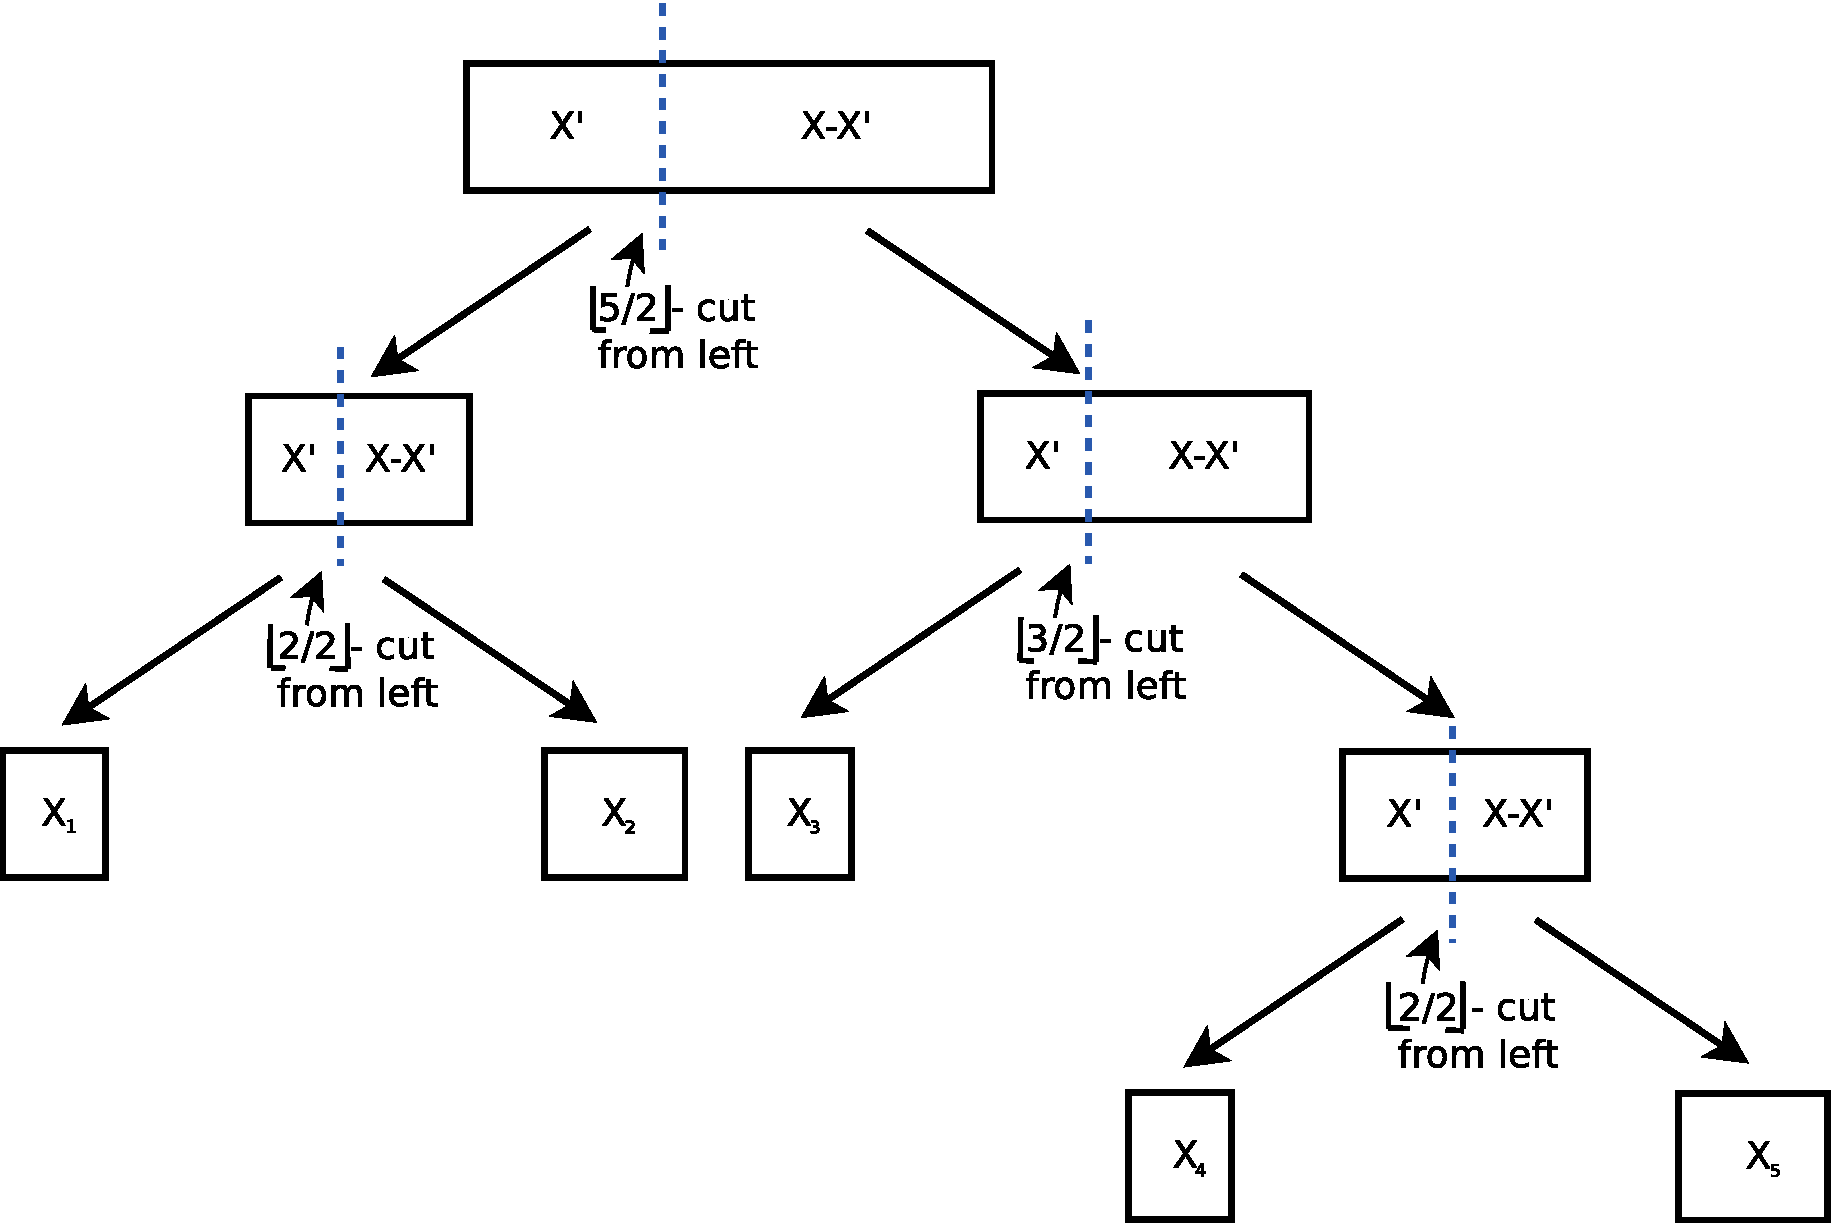
\includegraphics[width=380pt]{bilder/dcbsp.pdf}
   \caption{D$\&$C execution for $n=5$}
  	 \end{figure}
\begin{lem}
\label{dc1}
The Divide-$\&$-Conquer protocol is strategyproof for proportional protocols.
\end{lem}
\begin{proof} (similar to \cite{dc}:)\\
\newline
Assume two players $p_1$ and $p_2$ cutting a cake. Player $p_1$ is the cheater. The truthful $\nicefrac{1}{2}$ points are shown below, then by making a cut at $|$ would give $p_1$ and $p_2$ more than $\nicefrac{1}{2}$: 
$$l-----------p_1-|-p_2------------r$$ 
But if player $p_1$ moves his $\nicefrac{1}{2}$ point more to the left, he gets into the risk of
getting less than $\nicefrac{1}{2}$, if $|$ also moves due to his actions to the left. 
But if player $p_1$ moves his $\nicefrac{1}{2}$ point more to the right, he gets into the risk of
getting less than $\nicefrac{1}{2}$, if he crosses $p_2$'s $\nicefrac{1}{2}$ point. This proof can be extended to $n>2$.
\end{proof}
\begin{bezeichnungen}
According to Theorem \ref{thm5} and Theorem \ref{dc1} and Theorem \ref{dc2} 
Even $\&$ Paz Divide-$\&$-Conquer is strategyproof for proportional protocols, strategyproof game-theoretical strategyproof and weak strategyproof.
\end{bezeichnungen}
\newpage
 	 
%%%%%%%%%%%%%%%%%%%%%%%%%%%%%%%%%%%%%%%%%%%%%%%%%%%%%%%%%%%%%%%%%%%%%%%%%%%%%%%%%%%%%%%%%%%%%%%%%%%%%%%%%%%%%%%%
%%%%%%%%%%%%%%%%%%%%%%%%%%%%%%%%%%%%%%%%%%%%%%%%%%%%%%%%%%%%%%%%%%%%%%%%%%%%%%%%%%%%%%%%%%%%%%%%%%%%%%%%%%%%%%%%
%%%%%%%%%%%%%%%%%%%%%%%%%%%%%%%%%%%%%%%%%%%%%%%%%%%%%%%%%%%%%%%%%%%%%%%%%%%%%%%%%%%%%%%%%%%%%%%%%%%%%%%%%%%%%%%%
\section{Conclusion}
The strategyproofness in the context of cake-cutting has not been widely researched yet. In this work an overview over the occured definitions of the last five years is given. The applicability of them was proven. Hereby a proportional cake-cutting protocol is always weak and never strong strategyproof. For cake-cutting applicable definitions an overview over the correlation is given.\\
\newline
The well-known proportional cake-cutting protocols have been rewritten into a game-theoretic manner and analysed on whether a non-truthful strategy could yield a more advantageous situation for a non-truthful player. It was possible to approve game-theoretically that the only strategy which promises the best outcome is the strategy recommended by the protocol.\\
\begin{table}[htb]
\centering
 \renewcommand{\arraystretch}{1.5} 
\begin{tabular}{|l|c|c|c|c|c|}
\hline
$\:$Protocol & \multicolumn{1}{c|}{WSP} & GTSP & SP & SPP &SSP  \\
\hline
$\:$Cut $\&$ Choose & \Checkmark & \Checkmark  &\Checkmark & \Checkmark &  \XSolidBrush\\
\hline
$\:$Last-Diminisher & \Checkmark & \Checkmark & \Checkmark& \Checkmark &  \XSolidBrush\\
\hline
$\:$Lone-Chooser & \Checkmark & \Checkmark  &\Checkmark & \Checkmark &  \XSolidBrush\\
\hline
$\:$Lone-Divider & \Checkmark & \XSolidBrush  & \XSolidBrush &\XSolidBrush & \XSolidBrush \\
%\hline
%$\:$Cut your Own Piece & SPP & SP & \XSolidBrush & \Checkmark &SP& GSP \\
\hline
$\:$Divide-$\&$-Conquer & \Checkmark & \Checkmark &\Checkmark &\Checkmark &  \XSolidBrush \\
\hline
\end{tabular}
\caption{Overview: Strategyproofness of proportional cake-cutting protocols}\label{ov}
\end{table}

%%%%%%%%%%%%%%%%%%%%%%%%%%%%%%%%%%%%%%%%%%%%%%%%%%%%%%%%%%%%%%%%%%%%%%%%%%%%%%%%%%%%%%%%%%%%%%%%%%%%%%%%%%%%%%%%
%%%%%%%%%%%%%%%%%%%%%%%%%%%%%%%%%%%%%%%%%%%%%%%%%%%%%%%%%%%%%%%%%%%%%%%%%%%%%%%%%%%%%%%%%%%%%%%%%%%%%%%%%%%%%%%%
%%%%%%%%%%%%%%%%%%%%%%%%%%%%%%%%%%%%%%%%%%%%%%%%%%%%%%%%%%%%%%%%%%%%%%%%%%%%%%%%%%%%%%%%%%%%%%%%%%%%%%%%%%%%%%%%
\subsection{Related Work}
Recently, two papers with the focus on strategyproofness have been published. In \cite{chen:truth} they weakened the basic concepts of cake cutting by including the free disposal assumption, which can lead to a not complete allocation of the cake and allow only piecewise uniform valuations. The second restriction is indeed very hard. Their goal was to give a proportional, envy-free, polynomial and strong strategyproof protocol. In \cite{tamuz} the authors invented new procedures including a referee, who has full knowledge. This extension is a restriction of cake-cutting as well. They partly considered the case with indivisible items, where for example in \cite{Lipton} research in strategyproofness been done earlier, but is not practical applicable to cake-cutting. \cite{chen:truth} and \cite{tamuz} also researched truthfulness in expectation for randomized protocols.\\ \newline
In pie-cutting \cite{why} showed that a strategyproof and efficient mechanism must be dictatorial. The definition of strategyproofness in this paper is the strongest condition and is mostly used in economics, game theory or social choice theory. Also pie-cutting, slightly differs from cake-cutting, since the pie ist represented as a circular object and the cuts are wedges. The results for pie-  and cake-cutting do not carry over to each other, but the definition of strategyproofness does. \cite{pie} gave more details in the context of pie-cutting and strategyproofness. \\
\newline
The start of researching strategyproofness was \cite{brams}, where the authors introduced a fitting definition of strategyproofness (weak strategyproof in this work) and proved that two procedures called SP and EP are weak strategyproof.\\ A response on their work was a counterexample by \cite{ccc}. The authors argued that each proportional protocol is weak strategyproof. After admitting their mistake, in \cite{note} they restricted their first definition to cases with non-equal valuation functions and introduced a new general definition for strategyproof cake-cutting.\\
In \cite{dc} and in the revisited version of this work \cite{dc2} the authors focused on the Divide-and-Conquer protocol and showed that it is strategyproof for risk averse players. In the later work they call this property truth-inducing. \\ \cite{lindner:degrees} parallelised the Last-Diminisher and proved that this new protocol is also strategyproof for risk-averse players.%%%%%%%%%%%%%%%%%%%%%%%%%%%%%%%%%%%%%%%%%%%%%%%%%%%%%%%%%%%%%%%%%%%%%%%%%%%%%%%%%%%%%%%%%%%%%%%%%%%%%%%%%%%%%%%%
%%%%%%%%%%%%%%%%%%%%%%%%%%%%%%%%%%%%%%%%%%%%%%%%%%%%%%%%%%%%%%%%%%%%%%%%%%%%%%%%%%%%%%%%%%%%%%%%%%%%%%%%%%%%%%%%
%%%%%%%%%%%%%%%%%%%%%%%%%%%%%%%%%%%%%%%%%%%%%%%%%%%%%%%%%%%%%%%%%%%%%%%%%%%%%%%%%%%%%%%%%%%%%%%%%%%%%%%%%%%%%%%%
\section{Open Questions and Future Research}
%For two main listed reasons the influence of cooperative game theory is kept short in this work. One of them is the statement of Nash himself from \cite{Nash: non-cooperative Games, 1950} where he proposed, that each cooperative game can be displayed as a non-cooperative game with cooperation in the set of valid strategies. \\
%\begin{bsp}
%\label{bsp2}
%(Cooperative Cake-Cutting)\\
%After the win of the election in Turingville the member of President Church coalition wants to divide successfully the power in the country. Some of the members are aware of being unsatisfied with the outcome and so cooperate mutually to change the allocation.
%\end{bsp}
An interesting aspect would be to take a closer look on groupstrategyproofness. Hereby, groups have public valuations for group members.\\
\newline
Another approach about strategyproofness could be a consecutively allocation of several cakes. Then the cake-cutting-game could be interpreted as a repeated game. \\
Actually only a few game-theoretic methods are applied in this work. An a lot more intense research could yield towards different results and different applications in the field of cake-cutting. Some possible application field could be the Last Diminisher protocol where the players know their stage in the game or the Divide-$\&$-Conquer protocol with the focus on whether the participants can gain some advantages from knowing with how many players they are dividing a part of the cake and how many marks are on the left or right side of their mark.\\
More protocols like ''cut your own piece'' or other can be also analysed.\\
It would be interessting primary to search for strategies which fulfill the strategyproofness criterion but not the game-theoretic strategyproofness criterion.\\
The probability model that is used in this work is very simply, since even if the player $p_1$ cuts a cake in two pieces $\{X', X-X'\}$ with the value $v_1(X')=1-\epsilon$ and $v_1(X-X')=\epsilon$ the probability that player $p_2$ takes $X'$ or $X-X'$ is equal. In many application is this not reasonable for example in a divorce settlement allocation, if $X'$ is a Lamborghini and $X-X'$ the old carpet in the kitchen. There are valuations where it is possible, for example if the carpet was a gift from Elvis Presley and maybe even more money worth than the car. A further application could be to correlate the valuation of the cutter and the probability of the other players in taking this piece. 

\pagebreak

%%%%%%%%%%%%%%%%%%%%%%%%%%%%%%%%%%%%%%%%%%%%%%%%%%%%%%%%%%%%%%%%%%%%%%%%%%
%%%%%%%%%%%%%%%%%%%%%%%%%%%%%%% ENDE TEXTTEIL %%%%%%%%%%%%%%%%%%%%%%%%%%%%
%%%%%%%%%%%%%%%%%%%%%%%%%%%%%%%%%%%%%%%%%%%%%%%%%%%%%%%%%%%%%%%%%%%%%%%%%%

\clearpage
\thispagestyle{empty}
%\vspace*{\fill}g
\pagestyle{plain}
\bibliography{references.bib}
\bibliographystyle{apalike}
\thispagestyle{empty}
%\vspace*{\fill}g
\pagestyle{plain}
\clearpage

\listoffigures

\listoftables
\thispagestyle{empty}
%\pagebreak
\pagestyle{plain}
%\printindex
\end{document}